\chapter{Unfallerkennung im Pocket-Mode}
Dieses Kapitel beschäftigt sich mit der Weiterentwicklung der Unfallerkennung im Taschenmodus und mit der Implementierung neuer Funktionen sowie die Verifizierung dieser Änderungen. Es wird zuerst erwähnt, warum ein Pocket-Mode wichtig ist und welche Szenarien im Vergleich zum originalen Unfallerkennungsalgorithmus Unterschied machen würden.
Schließlich werden ein Paar Szenarien näher betrachtet und Verifikationsversuche geplant, durchgeführt und abschließend ausgewertet werden.

\section{Grund des Pocket-Modes}
Die Anzahl der App-Nutzer (Unfallerkennungsalgorithmus) lag im November 2021 bei ca. 1190. Die Anzahl der zugelassenen Motorräder zum gleichen Zeitraum betrugt in Deutschland ca. \SI{4,6}{\Million}. Um die Anzahl der App-Nutzer zu erhöhen, sollten die Bedürfnisse der Benutzern bekannt sein, damit diese durch erweiterte beziehungsweise neue Funktionen abgedeckt werden.

In diesem Sinne wurde eine Umfrage vom Spiegel-Institute im Auftrag von Bosch Help Connect im Zeitraum zwischen November und Dezember 2021 in vier Länder (Deutschland, Frankreich, Italien, Spanien) mit jeweils 333 Befragten durchgeführt.

Die zwei wichtigsten relevante Fragen waren:
\begin{itemize}
	\item Wofür nutzen Sie Ihr Smartphone während einer Fahrt mit dem Motorrad?
	\item Wo befindet sich aktuell Ihr Smartphone während der Fahrt normalerweise?
\end{itemize}
%************* Ergebnisse der Umfragen: Im Kommentar!! ************* %\\bosch.com\dfsrb\DfsDE\LOC\Wa2\BHCS\310_PJ-CL\025_Help_Connect\030_Marketing\110_UX\Nutzerwissen\Ergebnisse

Die Ergebnisse der Umfrage aus den vier Ländern lagen sehr nah zu einander, deswegen wird demnächst nur das Umfrageergebnis der deutschen Nutzern erläutert.

In der \autoref{fig:CalimotoUmfragePocketMode} ist das Ergebnis der Umfrage aus dem deutschen Markt dargestellt. 47\% der Befragten nutzen kein Smartphone während einer Fahrt, weil die Strecke bekannt ist oder weil sie Ihre Smartphones nicht am Lenker befestigen wollen. 70\% der Befragten haben Ihre Handys nicht am Motorrad oder am Lenker gehabt sondern in der (Hosen-)Tasche beziehungsweise im Rucksack. 
%- Grund: viele fahren nur kurze oder bekannte Strecken und wollen Ihre Handy nicht am Lenker befestigen (oder haben die Möglichkeit nicht). 

%(Figure von der Umfrage Calimoto). ->> Unfallerkennung laufen lassen, auch wenn das Handy in der Tasche ist.\\

%\autoref{fig:CalimotoUmfragePocketMode} zeigt die Daten...

\begin{figure}
	\centering
	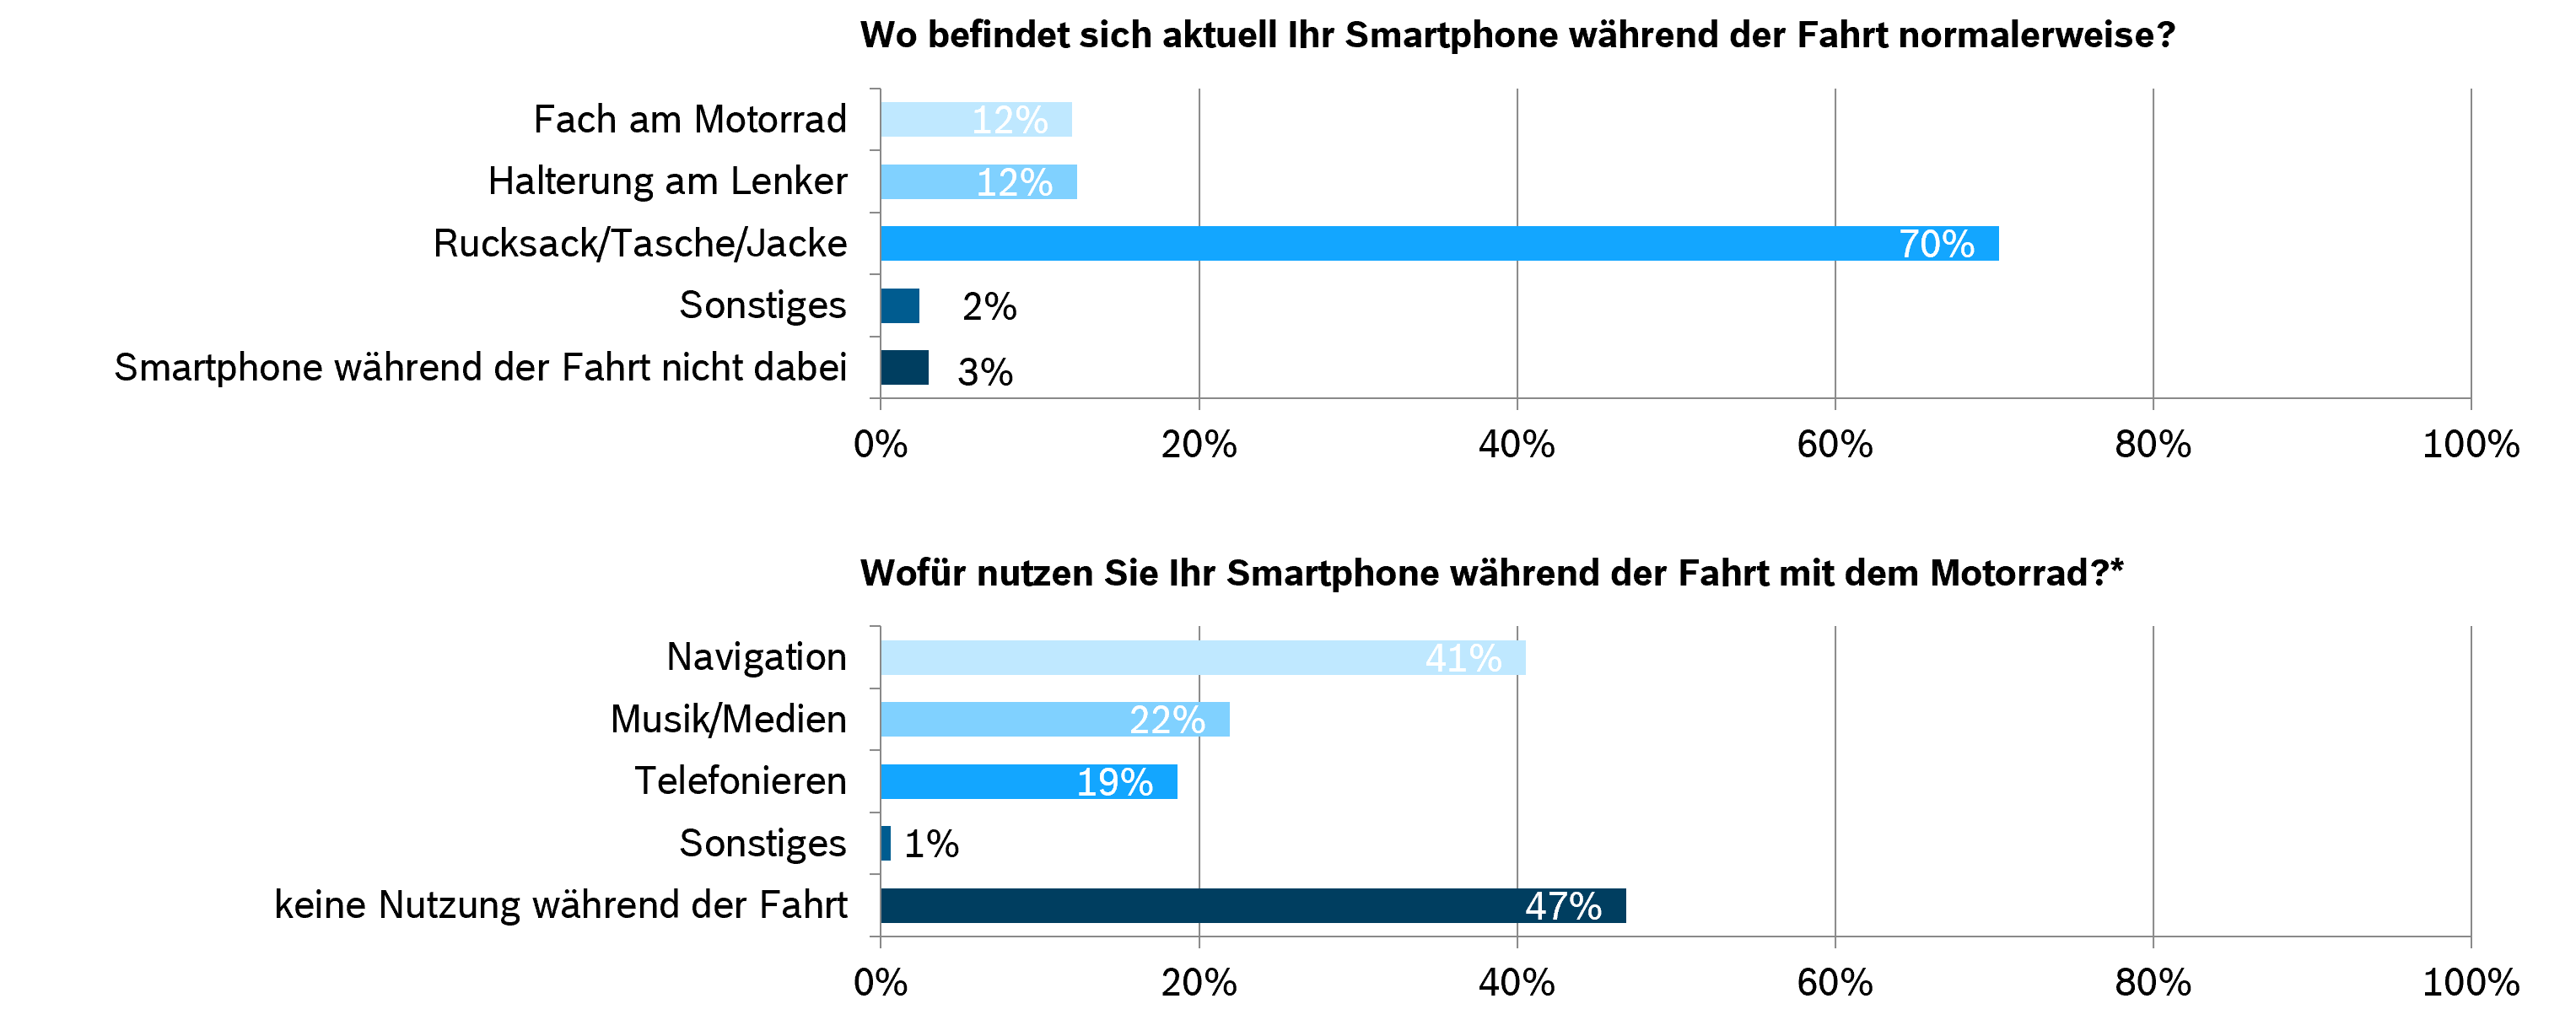
\includegraphics[width=\linewidth]{Bilder/SpiegelUmfragePocketMode.png}
	\caption{Ergebnisse der Umfrage vom Spiegelinstitute über das Taschenmodus}
	\label{fig:CalimotoUmfragePocketMode}
\end{figure}

Aus diesem Grund ist die Entwicklung einer Unfallerkennung im Pocket-Mode wichtig, um das Smartphone nicht mehr unbedingt am Lenker befestigt werden zu müssen. Die Weiterentwicklung der Unfallerkennung wird mit agilen Methoden erfolgt.

\section{Kritische Szenarien}
Im \autoref{abs:Unfallerkennungsalgorithmus} ist der Ablauf der aktuellen Unfallerkennungsalgorithmus sowie deren Parameter (z.B. TipOver) erläutert. Die Entwicklung des Pocket-Modes sollte auf keinen Fall zu Konflikten mit dem normalen Modus führen. Die bisherige Zuverlässigkeit des Algorithmus darf ebenso durch das Pocket-Mode nicht verringert werden, in dem ein im normalen Modus gut erkennbares Unfallszenario durch das Pocket-Mode übersehen wird.

Um solche Konflikte zu vermeiden, wird eine Liste der Use- sowie Edgecases vorbereitet, in der die Erwarteten Reaktion des aktuellen Algorithmus zum jeweiligen Szenario aufgelistet wird. Dadurch erfolgt eine Übersicht der möglichen Konflikten sowie der Fällen, wo ein falscher Alarm ausgelöst werden könnte, und gleich eine mögliche Gegenmaßnahme.

%Liste der Edge- und usecases mit einer Erklärung, warum diese kritisch sind und einen Vorschlag, was man dagegen tun kann.
Die \autoref{tab:EdgeCasesExcel} zeigt die Liste. Die Spalte \glqq Szenario\grqq{} enthält eine allgemeine Beschreibung des Szenarios, das auch unterteilt wird. In der Spalte \glqq Beschreibung\grqq{} ist eine nähere Erklärung des Szenarios erläutert.
Da das Verhalten des Smartphones in der Hosentaschen (am Oberschenkel) und am Oberkörper unterschiedlich sein könnte, werden diese separat betrachtet.
Die Spalte \glqq Erkennung durch den Algo\grqq{} berichtet, ob der aktuelle Algorithmus das entsprechende Szenario richtig erkennen wird (IO: In Ordnung, NIO: Nicht In Ordnung). Unter \glqq Bemerkungen\grqq{} ist eine weitere Erklärung des erwarteten Ergebnisses beschrieben. 
Unter der Bewegung des Oberkörpers fallen verschiedene Möglichkeit, z.B. seitliches Lehnen, was der Algorithmus problemlos erkennen würde und keine falsche Alarme auslöst.

Bei den kritischen Szenarien, wo der Algorithmus den Fall nicht richtig erkennen würde, ist eine mögliche Gegenmaßnahme zum Korrigieren der Algo\-rithmus-Ent\-scheid\-ung aufgeschrieben.
Einige Szenarien (z.B. Auf der Fußraste während einer Fahrt zu stehen) sollen ausführlich getestet werden, um die richtige Reaktion des Algorithmus zu analysieren und gegebenenfalls eine Gegenmaßnahme einzuplanen.

%\begin{figure}[H]
%	\centering
%	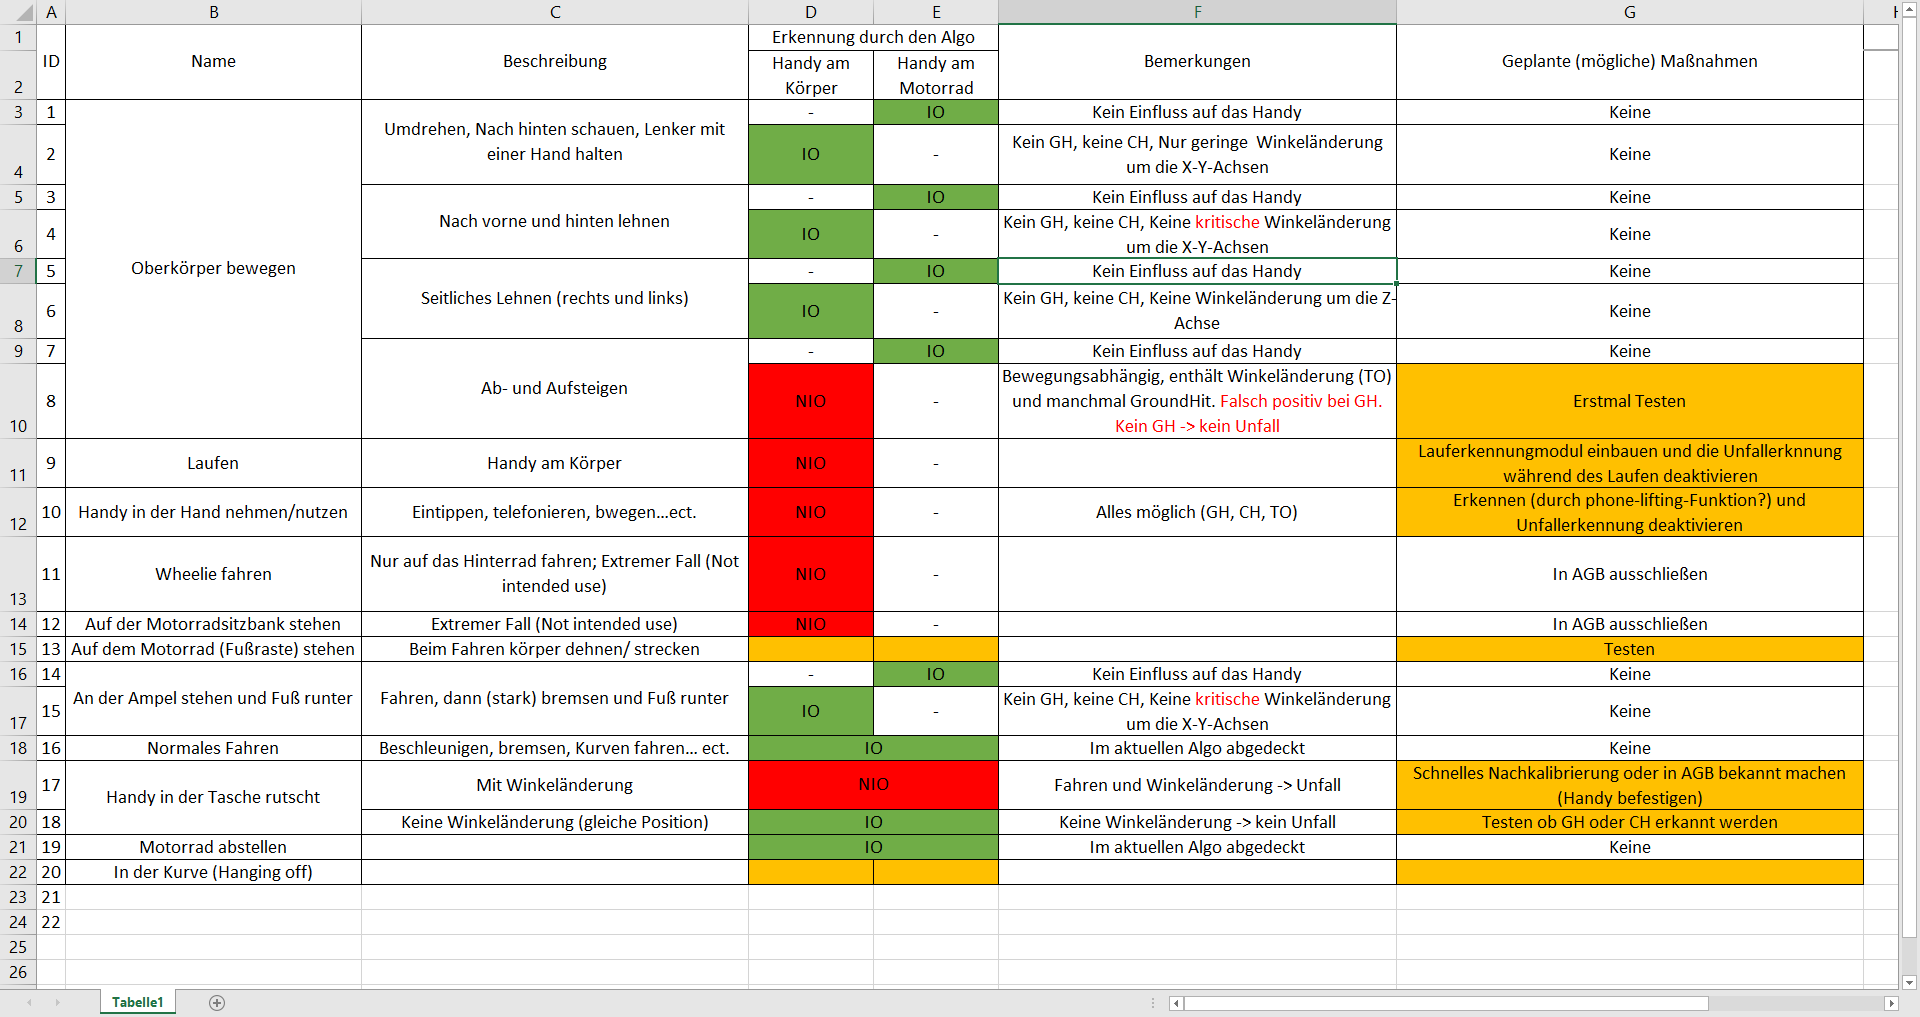
\includegraphics[width=\linewidth]{Bilder/EdgeCasesExcel.png} % TODO: Tabelle machen
%	\caption{Die Use- und Edgecases mit der erwarteten Reaktion des Algorithmus}
%	\label{fig:EdgeCasesExcel}
%\end{figure}
\begin{landscape}
	\footnotesize
	\begin{longtable}{|c|c|l|cc|l|l|}
		\caption{Die Use- und Edgecases mit der erwarteten Reaktion des Algorithmus}
		\label{tab:EdgeCasesExcel}
		\endfirsthead
		\endhead
		\hline
		&  &  & \multicolumn{2}{c|}{\begin{tabular}[c]{@{}c@{}}\\[-0.5em] Algo-Reaktion \\ (Erwartungen)\\[0.5em]\end{tabular}} &  &  \\ \cline{4-5}
		\multirow{-3}{*}{ID} & \multirow{-3}{*}{Szenrio} & \multirow{-3}{*}{Nähere Beschreibung} & \multicolumn{1}{c|}{\begin{tabular}[c]{@{}c@{}}Handy am \\ Körper\end{tabular}} & \begin{tabular}[c]{@{}c@{}}\\[-0.5em]Handy am \\ Motorrad\\[0.5em]\end{tabular} & \multirow{-3}{*}{Bemerkung} & \multirow{-3}{*}{Potenzielle Gegenmaßnahmen} \\ 
		\hline
		1 &  & \begin{tabular}[c]{@{}l@{}}\\[-0.5em]Umdrehen, Nach hinten \\ schauen,  Lenker mit \\ einer Hand halten\\[+0.5em]\end{tabular} & \multicolumn{1}{c|}{{\color[HTML]{009901} IO}} & - & \begin{tabular}[c]{@{}l@{}}Keine kritische  Winkel-\\ änderung um die X-Y-Achsen\end{tabular} & \multicolumn{1}{c|}{-} \\ \cline{1-1} \cline{3-7} 
		
		2 & \begin{tabular}[c]{@{}c@{}}Bewegung \\ des Körpers\end{tabular} & Nach vorne/hinten lehnen & \multicolumn{1}{c|}{{\color[HTML]{009901} IO}} & - & \begin{tabular}[c]{@{}l@{}}\\[-0.5em]Keine kritische  Winkel-\\ änderung um die X-Y-Achsen\\[+0.5em]\end{tabular} & \multicolumn{1}{c|}{-} \\ \cline{1-1} \cline{3-7} 
		
		3 &  & Seitliches Lehnen & \multicolumn{1}{c|}{{\color[HTML]{009901} IO}} & - & \begin{tabular}[c]{@{}l@{}}\\[-0.5em]Keine Winkeländerung \\ um die Z-Achse\\[+0.5em]\end{tabular} & \multicolumn{1}{c|}{-} \\ 
		\hline
		4 & Normale Fahrt & \begin{tabular}[c]{@{}l@{}}\\[-0.5em]Fahrt, Bremse, \\ Beschleunigung... usw.\\[+0.5em]\end{tabular} & \multicolumn{1}{c|}{{\color[HTML]{009901} IO}} & - & Bereits abgedeckt & \multicolumn{1}{c|}{-} \\ 
		\hline
		5 & Motorrad abstellen & \multicolumn{1}{c|}{-} & \multicolumn{1}{c|}{{\color[HTML]{009901} IO}} & - & Bereits abgedeckt & \multicolumn{1}{c|}{-} \\
		\hline
		6 & Hanging off & In der Kruve hängen & \multicolumn{1}{c|}{{\color[HTML]{009901} IO}} & - & \begin{tabular}[c]{@{}l@{}}\\[-0.5em]Keine ausreichende Winkel-\\ änderung für ein TipOver\\[+0.5em]\end{tabular} & \multicolumn{1}{c|}{-} \\ 
		\hline
		7 & Anhalten & \begin{tabular}[c]{@{}l@{}}\\[-0.5em]Starke Bremse nach \\ einer Fahrt und dann \\ Fuß runtersetzten\\[+0.5em]\end{tabular} & \multicolumn{1}{c|}{{\color[HTML]{009901} IO}} & - & \begin{tabular}[c]{@{}l@{}}Keine kritische Winkeländer-\\ ung um die X-Y-Achsen\end{tabular} & \multicolumn{1}{c|}{-} \\ 
		\hline
		8 & \begin{tabular}[c]{@{}c@{}}Ab- und \\ Aufsteigen\end{tabular} & \multicolumn{1}{c|}{-} & \multicolumn{1}{c|}{{\color[HTML]{FE0000} NIO}} & - & \begin{tabular}[c]{@{}l@{}}\\[-0.5em]Bewegungsabhängig, \\ enthält Winkeländerung \\ (TO)\\[+0.5em]\end{tabular} & Ausführliches Testen \\ 
		\hline
		9 & Laufen & \multicolumn{1}{c|}{-} & \multicolumn{1}{c|}{{\color[HTML]{FE0000} NIO}} & - & \begin{tabular}[c]{@{}l@{}}Im Taschenmodus sehr \\ wahrcheinlich\end{tabular} & \begin{tabular}[c]{@{}l@{}}\\[-0.5em]Lauferkennung einbauen \\ und die Unfallerknnung \\ während des Laufen de-\\ aktivieren\\[+0.5em]\end{tabular} \\ 
		\hline
		10 & \begin{tabular}[c]{@{}c@{}}Nutzung des \\ Smartphones\end{tabular} &  & \multicolumn{1}{c|}{{\color[HTML]{FE0000} NIO}} & - & \multicolumn{1}{c|}{-} & \begin{tabular}[c]{@{}l@{}}\\[-0.5em]Erkennung durch das \\ phone-lifting-Funktion\\[+0.5em]\end{tabular} \\ 
		\hline				
		11 & \begin{tabular}[c]{@{}c@{}}\\[-0.5em]Auf der Fußrasste \\ stehen\\[+0.5em]\end{tabular} & Stehend fahren & \multicolumn{1}{c|}{{\color[HTML]{010066} Testen}} & - & \multicolumn{1}{c|}{-} & Ausführliches Testen \\ 
		\hline
		12 & \begin{tabular}[c]{@{}c@{}}\\\\Rutschung des\\ Handys in der \\ Tasche\end{tabular} & Starke Winkeländerung & \multicolumn{2}{c|}{{\color[HTML]{FE0000} NIO}} & \begin{tabular}[c]{@{}l@{}}Fahrt und Winkeländerung \\ verursacht Unfallerkennung\end{tabular} & \begin{tabular}[c]{@{}l@{}}Schnelles Nachkalibrierung \\ oder in AGB bekannt machen \\ (Handy befestigen)\end{tabular} \\ \cline{1-1} \cline{3-7}
		
		13 &  & \begin{tabular}[c]{@{}l@{}}\\[-0.5em]Keine Winkeländerung \\ (keine Umdrehung)\\[+0.5em]\end{tabular} & \multicolumn{1}{c|}{{\color[HTML]{010066} Testen}} & - & \multicolumn{1}{c|}{-} & Ausführliches Testen \\ 
		\hline
		14 & Wheelie fahren & Auf das Hinterrad fahren & \multicolumn{2}{c|}{{\color[HTML]{FE0000} NIO}} & \begin{tabular}[c]{@{}c@{}}\\[-0.5em]Extremer Fall\\  (Not intended use)\\[+0.5em]\end{tabular} & In AGB ausschließen \\ 
		\hline
		15 & \begin{tabular}[c]{@{}c@{}}Auf der Motorrad-\\ sitzbank stehen\end{tabular} & \multicolumn{1}{c|}{-} & \multicolumn{2}{c|}{{\color[HTML]{FE0000} NIO}} & \begin{tabular}[c]{@{}c@{}}\\[-0.5em]Extremer Fall\\  (Not intended use)\\[+0.5em]\end{tabular} & In AGB ausschließen \\ 
		\hline
	\end{longtable}
\end{landscape}
Nach einer internen Statistik ist das Laufen ein häufiger Grund von den falschen Alarmauslösungen, deswegen ist eine Lauferkennung zur Verbesserung der Zuverlässigkeit sehr wichtig.

\section{Lauferkennung} \label{sec:Lauferkennung}
In der bereits bestehenden Version des Algorithmus ist davon ausgegangen, dass das Smartphone am Lenker befestigt wird. Wenn die Person das Handy nach einer Fahrt in die Hosen- beziehungsweise Jackentasche einsteckt und fängt an zu laufen, wird öfters einen falschen Alarm (falsch-positiv) ausgelöst, da das Laufen im bisherigen Algorithmus nicht berücksichtigt wurde.
Wenn die Unfallerkennung im Pocket-Mode verwendet wird, ist stark zu erwarten, dass die Person nach einer Fahrt oder während einer Pause (z.B. Tankpause) vergisst (oder ignoriert), die Unfallerkennung zu deaktivieren, und mit dem Smartphone an sich läuft. Das führt dazu, dass die Anzahl der falschen Alarmen im Pocket-Mode wesentlich steigt.

Diese Arbeit beschäftigt sich im Teil mit der Implementierung der Lauferkennung. Das Ziel dahinter ist das Laufen zu erkennen und die Unfallerkennung temporär zu deaktivieren, damit die falsche Alarme verhindert werden.
In diesem Kapitel werden die Entwicklungsschritte der Lauferkennung erläutert.

%% Generated using matlabfrag
% Version: v0.6.16
% Version Date: 04-Apr-2010
% Author: Zebb Prime
%
%% <text>
%
\providecommand\matlabtextA{\color[rgb]{0.150,0.150,0.150}\fontsize{11}{11}\selectfont\strut}%
\psfrag{Time}[tc][tc]{\matlabtextA Time}%
%
%% </text>
%
%% <xtick>
%
\def\matlabfragNegXTick{\mathord{\makebox[0pt][r]{$-$}}}
%
\providecommand\matlabtextB{\color[rgb]{0.150,0.150,0.150}\fontsize{10}{10}\selectfont\strut}%
\psfrag{000}[ct][ct]{\matlabtextB $25$}%
\psfrag{001}[ct][ct]{\matlabtextB $30$}%
\psfrag{002}[ct][ct]{\matlabtextB $35$}%
\psfrag{003}[ct][ct]{\matlabtextB $40$}%
\psfrag{004}[ct][ct]{\matlabtextB $45$}%
%
%% </xtick>
%
%% <ytick>
%
\psfrag{005}[rc][rc]{\matlabtextB $-5000$}%
\psfrag{006}[rc][rc]{\matlabtextB $-4000$}%
\psfrag{007}[rc][rc]{\matlabtextB $-3000$}%
\psfrag{008}[rc][rc]{\matlabtextB $-2000$}%
\psfrag{009}[rc][rc]{\matlabtextB $-1000$}%
\psfrag{010}[rc][rc]{\matlabtextB $0$}%
\psfrag{011}[rc][rc]{\matlabtextB $1000$}%
%
%% </ytick>

\begin{figure}
	\centering
	\psfragfig[width=\textwidth]{Bilder/LaufenMuster}
	\caption{Beispiel eines Beschleunigungssignal beim Laufen}
	\label{fig:LaufenMuster}
\end{figure}
In der \autoref{fig:LaufenMuster} ist ein Beispielsignal aus dem Beschleunigungssensor im Smartphone während des Laufens abgebildet. Die Person kann bis zu zwei Schritte pro Sekunde im Schnitt zurücklegen. In der Grafik können die Peaks innerhalb einer Sekunde aufgezählt werden und die durchschnittliche Anzahl der Schritten kann ermitteln werden. Wenn diese unter zwei pro Sekunde liegt, ist vom Laufen auszugehen, da ein Motor so wenige Umdrehungen pro Sekunde nicht schafft. Im nächsten Abschnitt werden diese Peaks aufgezählt, um die Anzahl der Schritten beziehungsweise Umdrehungen zu ermitteln.
%
\subsection{Spitzendzähler} \label{abs:PeaksAufzaehlen} %was ist ein Schritt? Schritt ist eine Beinbewegung. 1 Hz ist ein Schritt

Wie bereits erwähnt wurde, kann die Person bis zu zwei Schritte pro Sekunde laufen. D.h. aus einem typischen Laufsignal (z.B. \autoref{fig:LaufenMuster}) soll maximal zwei Schritte pro Sekunde aufgezählt werden.
Es soll ein System implementiert werden, das die Anzahl der Schritten beziehungsweise Spitzen aufzählt und der Mittelwert pro Sekunde zurückgibt. Zur Vereinfachung der Implementierung wird eine Simulink-Testumgebung (\autoref{fig:Lauferkennung_Peaks_Testbeispiel}) aufgebaut, in der ein bekanntes Sinussignal generiert, dargestellt und verarbeitet wird.
\begin{figure}
	\centering
	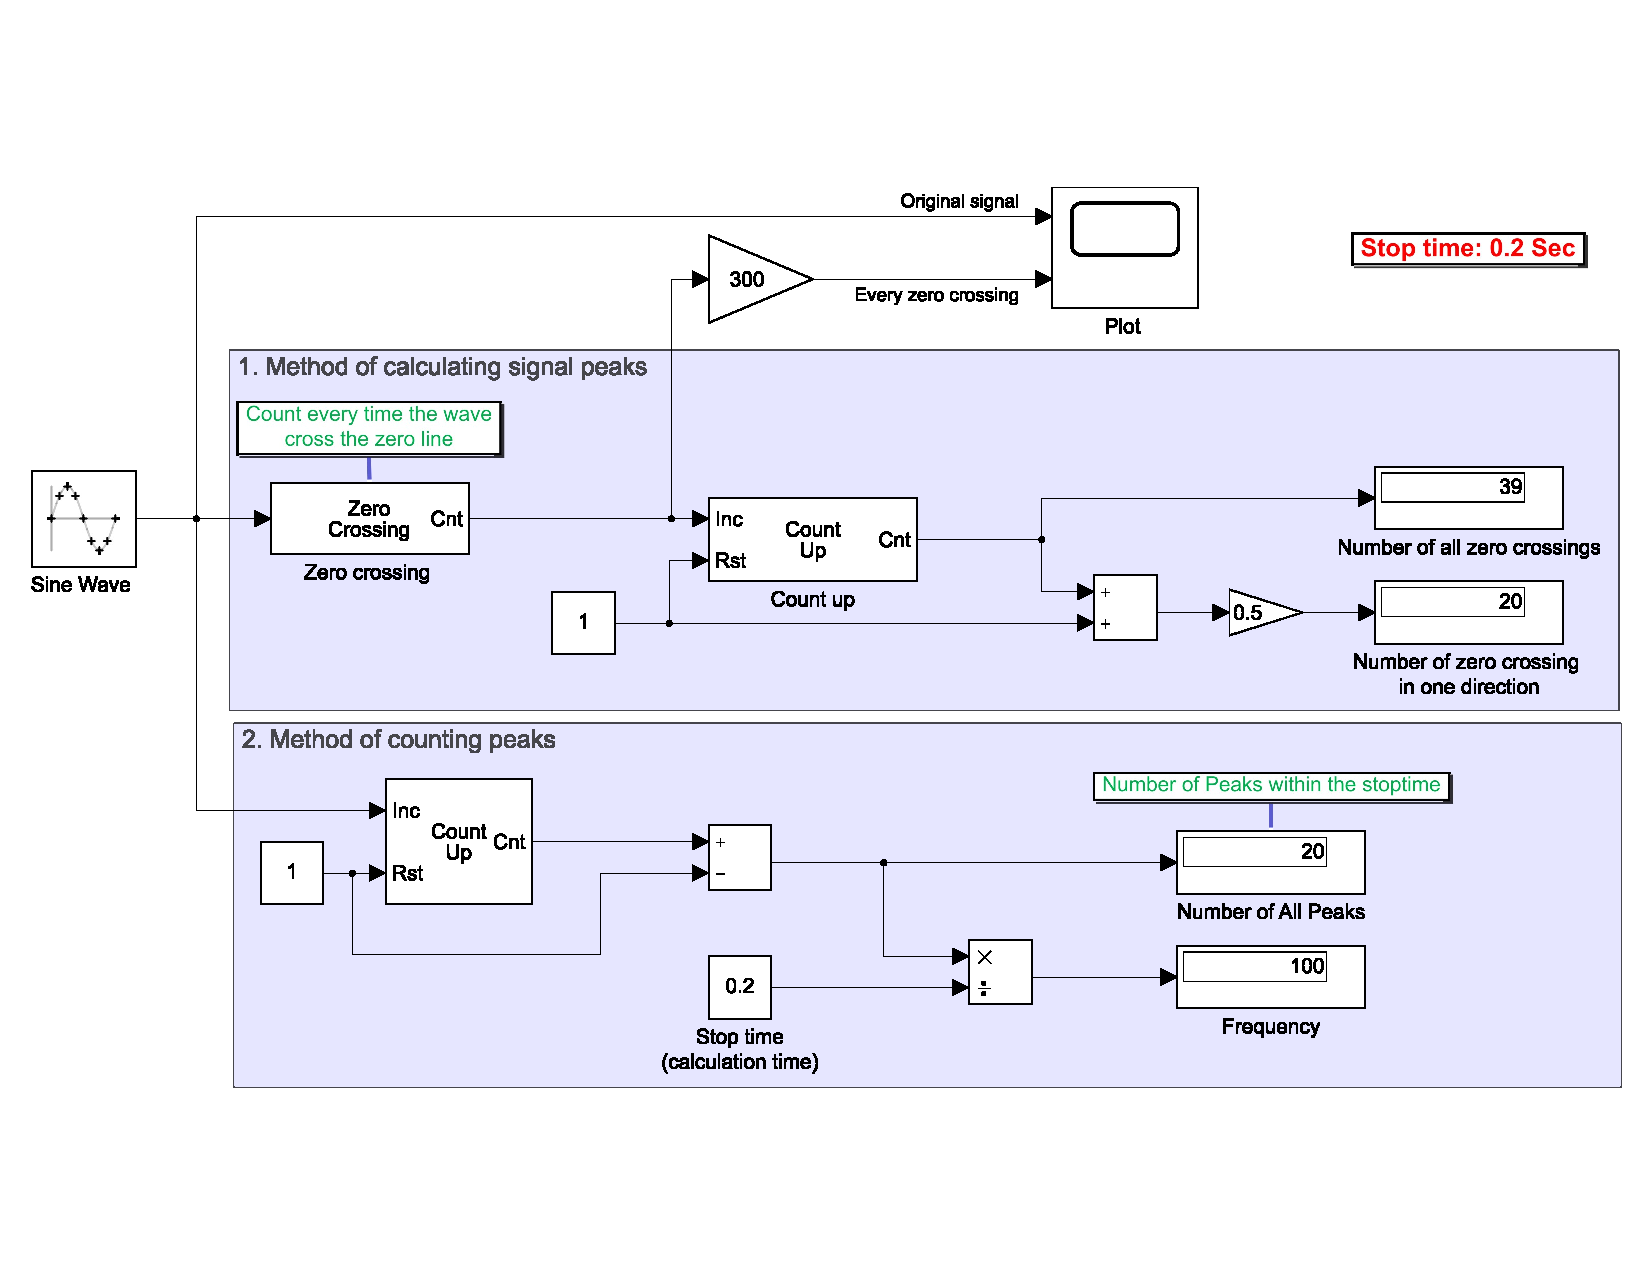
\includegraphics[width=0.8\linewidth]{Bilder/TestModellLauferkennungSpitzenzaehler.pdf}
	\caption{Testmodel der Lauferkennung - Spitzenzähler}
	\label{fig:Lauferkennung_Peaks_Testbeispiel}
\end{figure}
Das generierte Sinussignal hat eine Amplitude von 325 und eine Frequenz von \SI{100}{\hertz} und lässt sich mithilfe eines Scopes (Simulink-Block) in der \autoref{fig:Lauferkennung_Peaks_SinusSignal} (blau) darstellen sowie wie oft das Signal die x-Achse überschneidet (rot). Aus der Grafik ist die Anzahl der Peaks einfach zu ermitteln und diese beträgt in diesem Fall \SI{100}{\hertz} umgerechnet.

%Die \autoref{fig:Lauferkennung_Peaks_SinusSignalGenerator} zeigt die Spezifikationen des generierten Signals und die  stellt  das entsprechende Signal grafisch dar sowie 
%Eine zeitliche Frequenz wird folgendes berechnet:\\
%$Freq_Hz = \frac{Freq_(rad/sec)}{2\pi}$
%\begin{figure}[H]
%	\centering
%	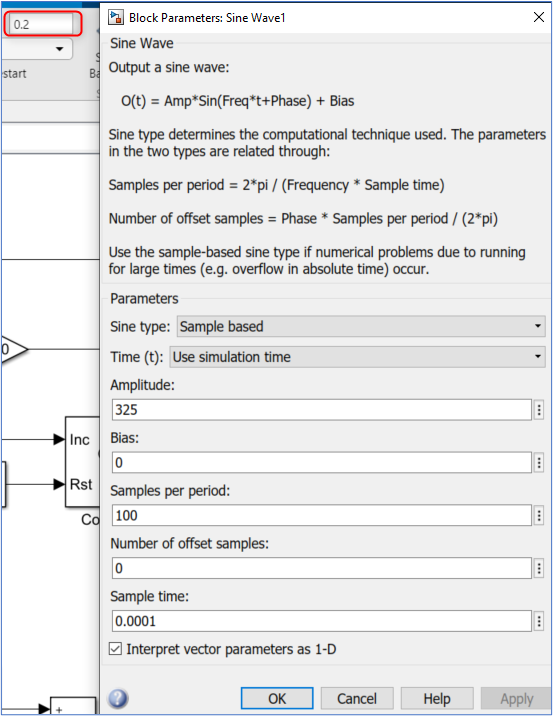
\includegraphics[width=0.5\linewidth]{Bilder/Lauferkennung_Peaks_SinusSignalGenerator.png}
%	\caption{Testbeispiel - Lauferkennung - Sinussignalgenerator - Spezifikationen}
%	\label{fig:Lauferkennung_Peaks_SinusSignalGenerator}
%\end{figure}
\begin{figure}
	\centering
	\psfragfig[width=\textwidth]{Bilder/0B_Lauferkennung_SinusPeaks}
	\caption{Darstellung des im Testmodel der Lauferkennung generierten Sinussignal sowie jede Überschneidung der x-Achse}
	\label{fig:Lauferkennung_Peaks_SinusSignal}
\end{figure}
Die \autoref{fig:Lauferkennung_Peaks_Testbeispiel} zeigt eine Testumgebung, in dem zwei Methoden zum Spitzenzähler implementiert wurden.

In der ersten (oberen) Methode wird die Funktion \glqq Zero Crossing\grqq{} verwendet. Diese zählt wie oft das Signal die x-Achse überquert. Dieses Model liefert das richtige erwartete Ergebnis, wenn das Signal um die x-Achse dargestellt ist, und hilft allerdings nicht, wenn das Signal ein Offset hat (Verschiebung auf der y-Achse), da in diesem Fall das Signal die x-Achse je nach der Amplitude nicht mehr überschneidet. Das führt dazu, dass das Ergebnis nicht mehr zuverlässig ist.

Eine zweite Methode hat sich ergeben, dass die Funktion \glqq Counter up\grqq{} in dem Model verwendet wird. Dieses Block zählt wie oft das Signal in die positive Richtung geht. Die neue Implementierung hat ein zuverlässiges Ergebnis im Vergleich zum vorherigen Model geliefert.

Beim Einsetzen des gleichen Vorgehens beziehungsweise Model auf das echte Laufsignal (\autoref{fig:LaufenMuster}) wird eine Frequenz von ca. \SI{11}{\hertz} beim Laufen zurückgegeben, was eigentlich nicht wahr ist, da der Mensch keine \SI{11}{Schritte pro Sekunde} zurücklegen kann.

Nach weiteren Auswertungen und Forschungen wird der Grund des Fehlers entdeckt. Es liegt an den Unterschied zwischen dem einfachen generierten Sinussignal und dem echten Laufsignal. Das echte Signal hat im Vergleich zum Generierten viele Störungen (Rauschen). Diese lassen sich durch das gedachte Model nicht ausfiltern oder ignorieren, was zu einem falschen Ergebnis führt. Die \autoref{fig:Skizze_IdealUndEchtSignal} stellt ein gutes Beispiel dieser Unterschied dar, in dem die Rauschen die Anzahl der Spitzen erhöhen.

Die \autoref{fig:Skizze_IdealUndEchtSignal} zeigt zwei sinusförmige Signalen. Die obere Grafik stellt ein einfaches Signal mit einer Frequenz von ungefähr $f = \SI{5,5}{\hertz}$ und die Untere ein komplexes Signal dar.
Das Model hat für das untere Signal \SI{19}{Spitzen pro Sekunde} geliefert, was die Wahrheit nicht entspricht.

%\begin{figure} % TODO: Vektorgrafik
%	\centering
%	\begin{subfigure}{\textwidth}
%		\centering
%		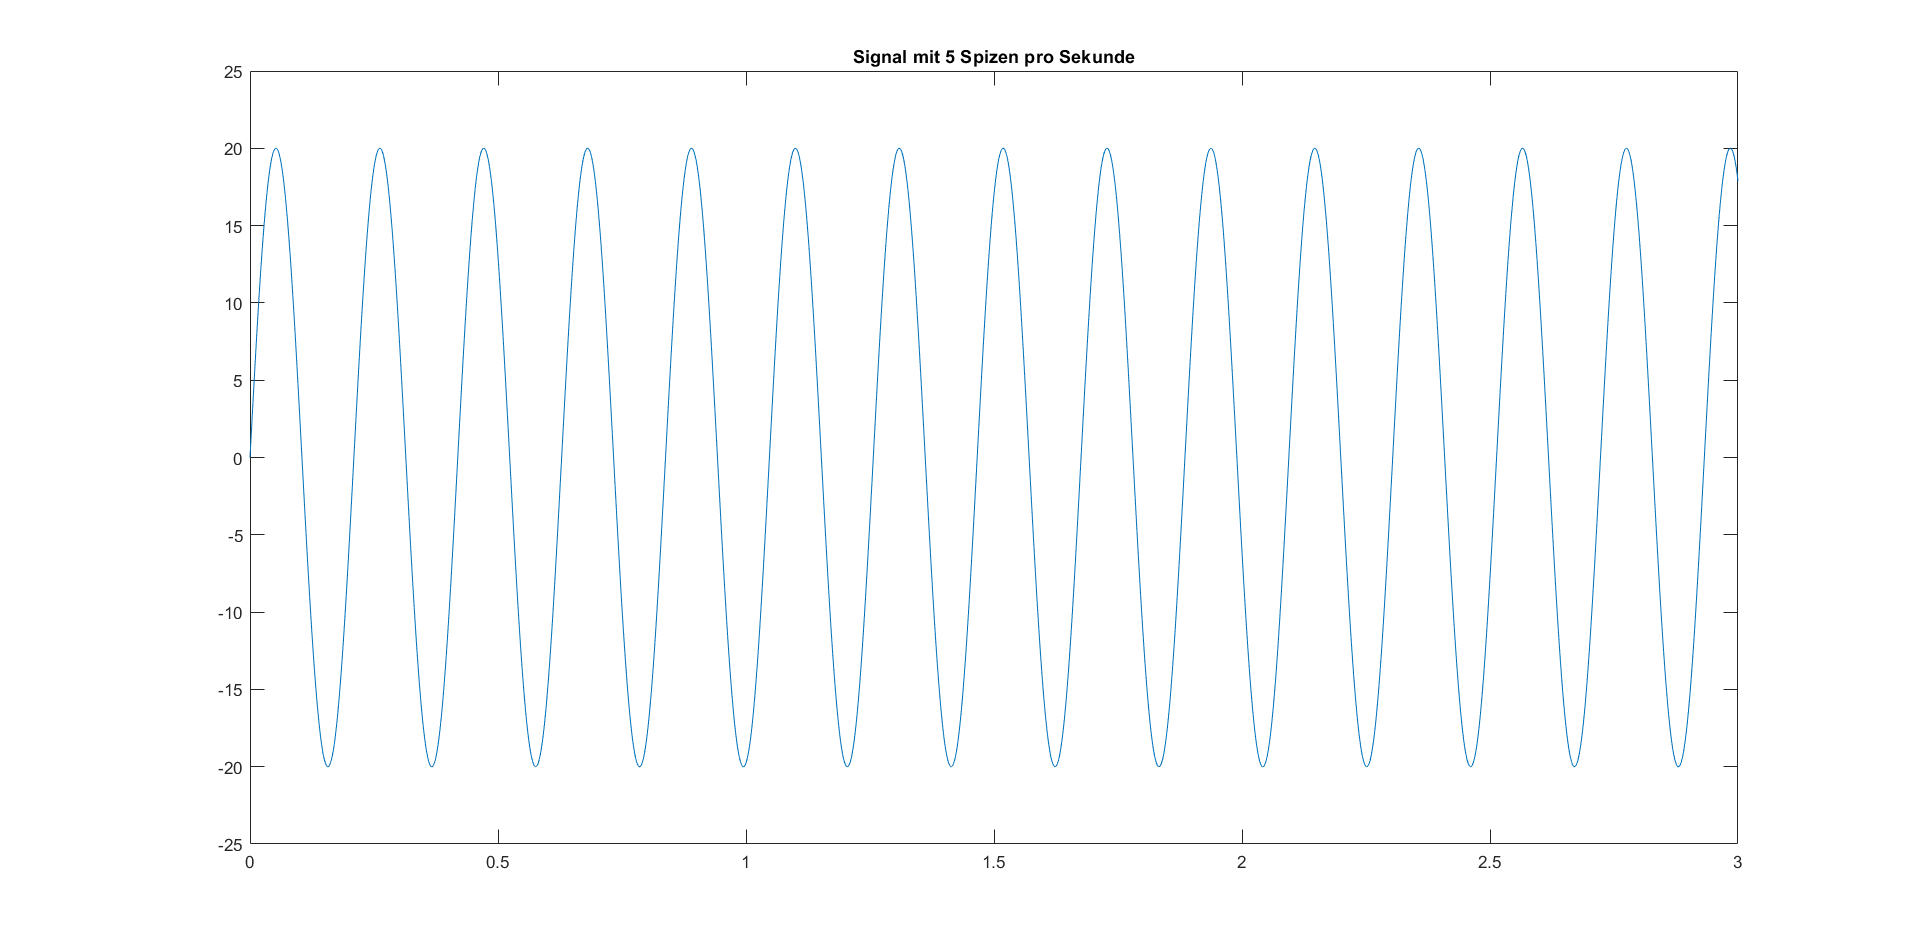
\includegraphics[width=\textwidth]{Bilder/einfachesSignalBeispiel.png}
%		\caption{Beispiel eines einfaches Signal}
%%		\label{fig:einfachesSignalBeispiel}
%	\end{subfigure}
%	\hfill
%	\begin{subfigure}{\textwidth}
%		\centering
%		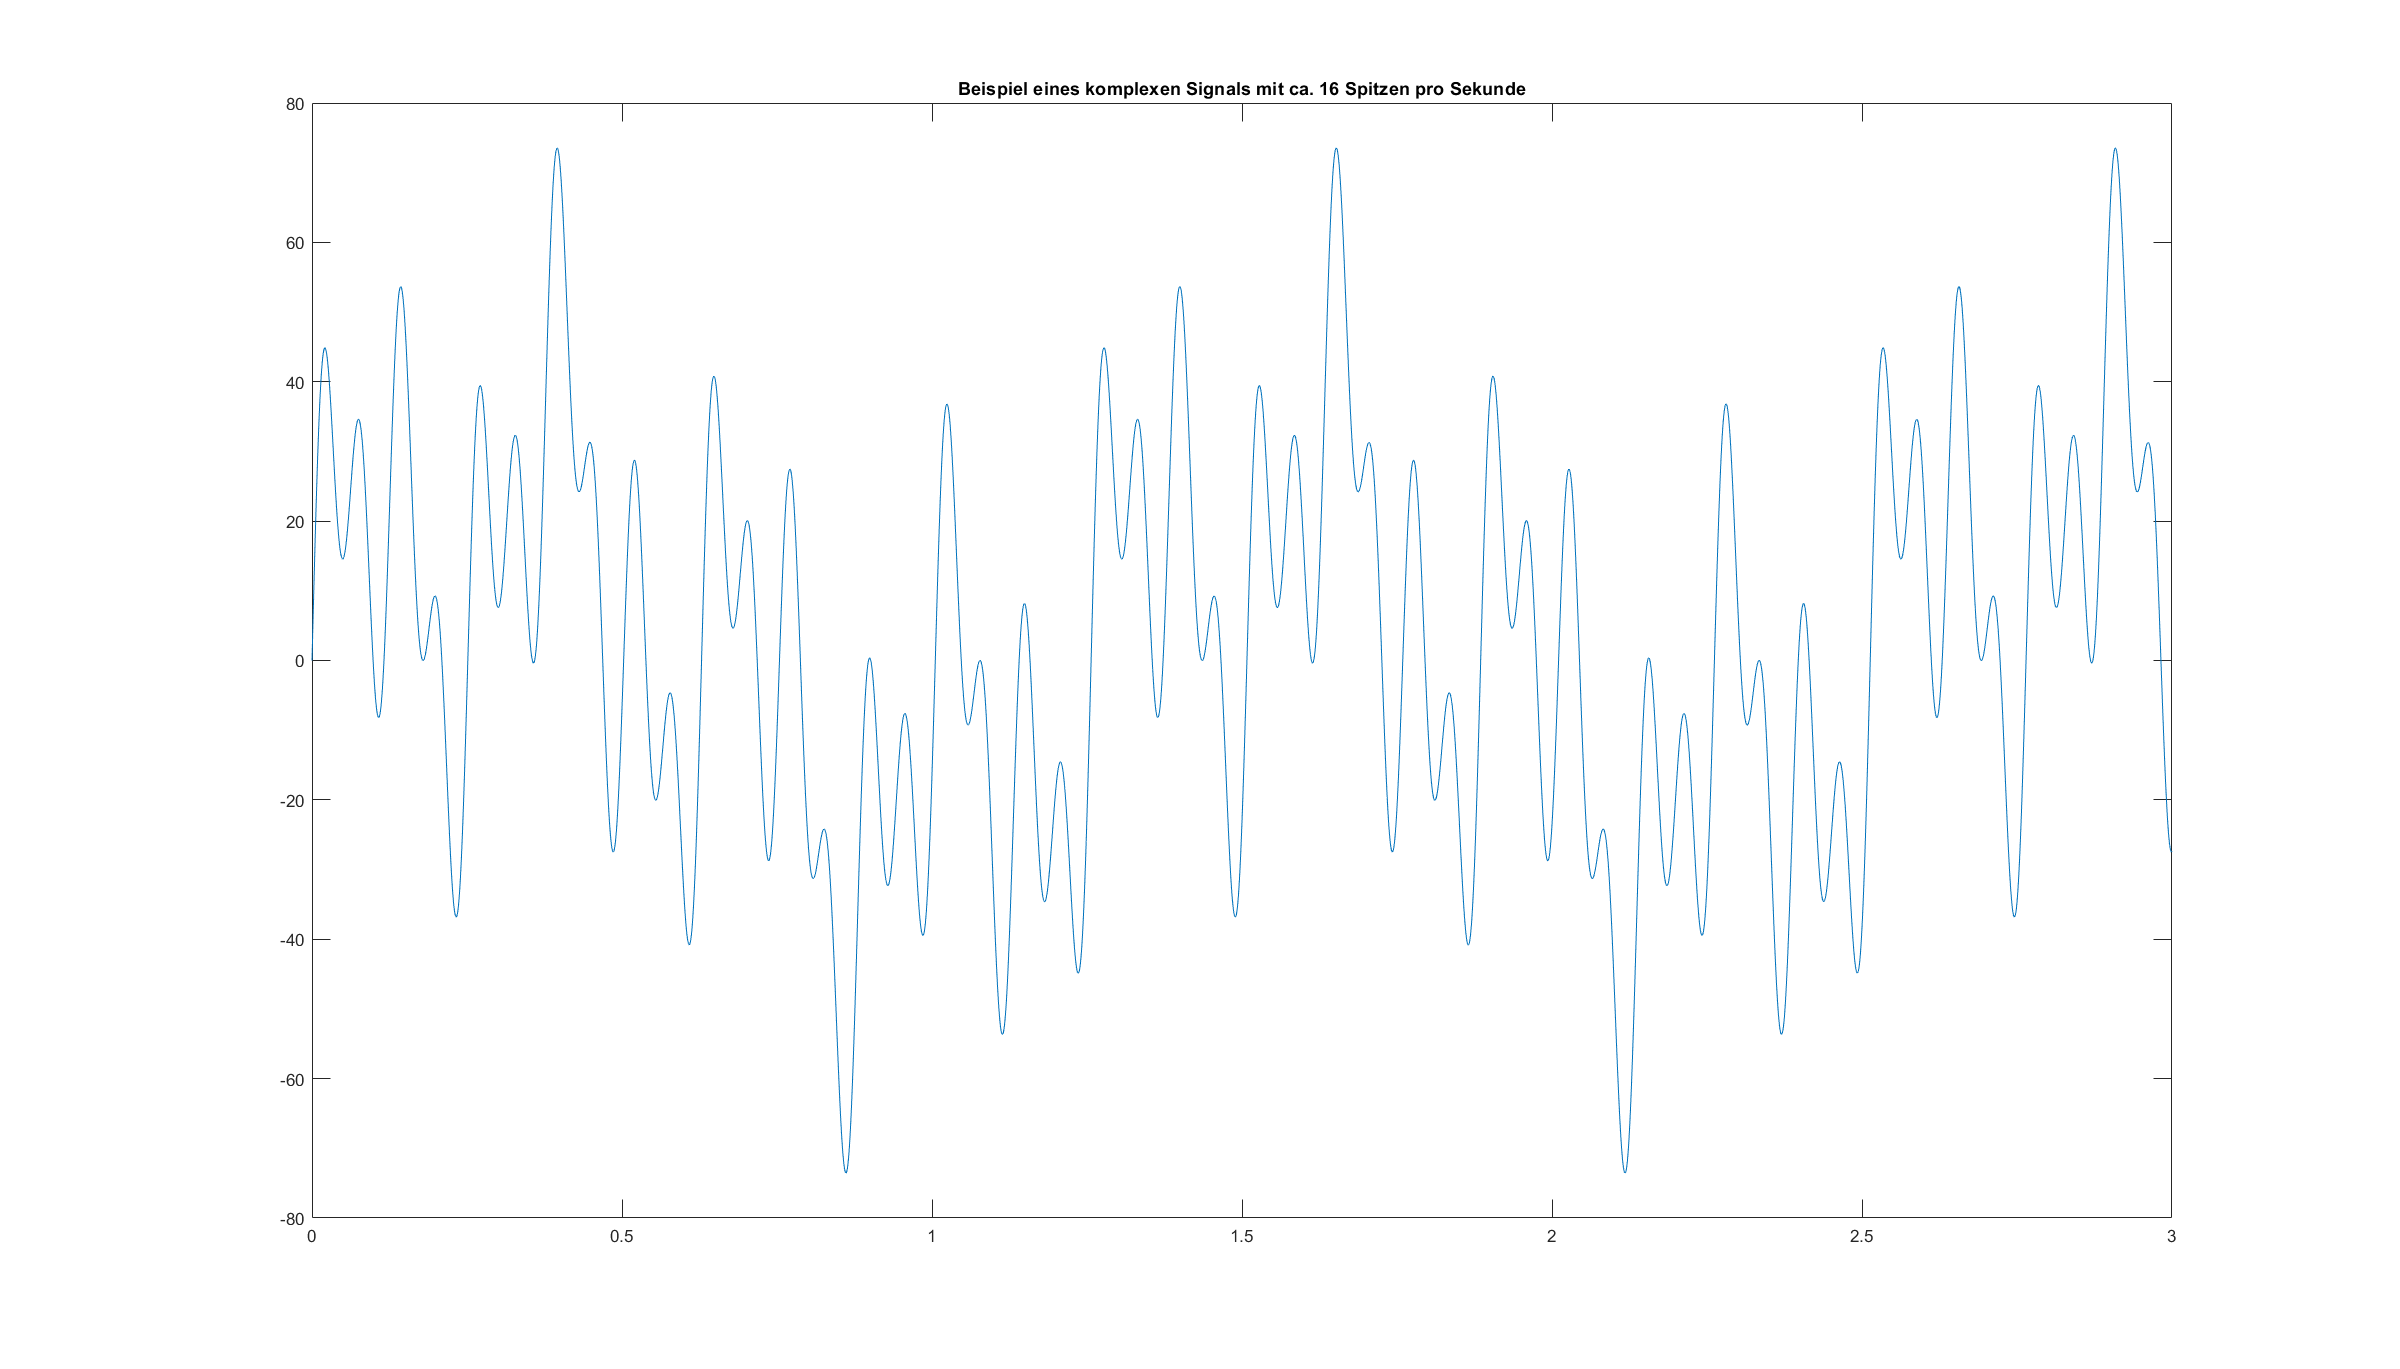
\includegraphics[width=\textwidth]{Bilder/komplexSignalBeispiel.png}
%		\caption{Beispiel eines komplexes Signal}
%%		\label{fig:komplexSignalBeispiel}
%	\end{subfigure}
%	\caption{Skizze eines einfaches ideales Signal sowie eines komplexeres Signal}
%%	\label{fig:Skizze_IdealUndEchtSignal}
%\end{figure}

\begin{figure}
	\centering
	\subfloat[Beispiel eines einfaches Signal]{
		\psfragfig[width=0.49\textwidth]{Bilder/0B_einfachesSignalBeispiel}\label{fig:einfachesSignalBeispiel}
	}
	\hfill
	\subfloat[Beispiel eines komplexes Signal]{	
		\psfragfig[width=0.49\textwidth]{Bilder/0B_komplexSignalBeispiel}\label{fig:komplexSignalBeispiel}
	}
	\caption{Skizze eines einfaches ideales Signal sowie eines komplexeres Signal}
	\label{fig:Skizze_IdealUndEchtSignal}
\end{figure}

Da der Spitzenzähler nicht zuverlässig funktioniert, ist eine bessere Idee notwendig. 


\subsection{Frequenzbasierte Lauferkennung}

Das Laufsignal stellt ein wiederholtes Muster (Pattern) durch die Fußbewegungen dar, was auch durch eine Frequenzermittlung erkannt werden kann.
Es soll ein Model gegeben werden, das diese Frequenz ermitteln und auswerten kann.
Analog zum \autoref{abs:PeaksAufzaehlen} wird hier nochmal eine neue Hypothese festgelegt, die durch einem Testsystem überprüft werden soll.

Die Hypothese: Die Frequenz während des Laufens sollte kleiner als \SI{2}{\hertz} sein und beim Fahren über \SI{7}{\hertz}. Wenn eine Frequenz von über \SI{7}{\hertz} ermittelt wird, ist eine Laufaktivität ausgeschlossen, da ein Mensch auf keinen Fall \SI{7}{Schritte} innerhalb einer Sekunde zurücklegen kann. Die Fahrfrequenz ist durch die Motorumdrehungen entstanden. 

Die Transformation vom Zeitbereich zum Frequenzbereich wird durch eine FFT erfolgt.
Die App der Unfallerkennung hat eine Abtastrate von $f_s = \SI{100}{\hertz}$ und nimmt \SI{100}{Messwerte pro Messsekunde} auf.
Bezogen auf die Nyquist-Frequenz (\autoref{gl:Nyquist-Frequenz}) lässt sich die minimale erkennbare Frequenz (Bandbreite) $f_n = \SI{50}{\hertz}$ geben.

\subsubsection{Spectrum Analyzer}
In der \autoref{fig:Lauferkennung_Freqbasiert_TestBeispiel_SinussignalGenerator} sind die generierten Sinussignale mit den Frequenzen $f=\SI{23,8}{\hertz}$, $f=\SI{47,8}{\hertz}$ und $f=\SI{1,1}{\hertz}$ zu sehen, die summiert werden, damit eine Komplexes Signal erstellt wird. Die drei Sinussignale sowie deren Summe sind in der \autoref{fig:Testsignal_AllViews} dargestellt.

Danach wird in diesem Model ein Block \glqq Spectrum Analyzer\grqq{} als Referenz verwendet, was die Grundfrequenzen des komplexen Signals zurückgibt. Der Benutzer kann die Spezifikationen vom \glqq Spectrum Analyzer\grqq{} einstellen. Die Ausgabe vom \glqq Spectrum Analyzer\grqq{} ist in der \autoref{fig:Lauferkennung_Freqbasiert_SpektrumAnalyzerAusgabe_gezoomt} veranschaulicht. In der Oberen Grafik werden die Intensität der Frequenz(en) (auch Spektrum genannt) abgebildet und in der unteren Grafik eine 3D-Darstellung \glqq Frequenz-Zeit-Intensität\grqq{} (Spektrogramm), wobei die Farbe die Intensität repräsentiert. Wenn die Abbildung näher betrachtet wird, sind die Grundfrequenzen von $f=\SI{23,8}{\hertz}$, $f=\SI{47,8}{\hertz}$ und $f=\SI{1,1}{\hertz}$ gut sichtbar.

\begin{figure}
	\centering
	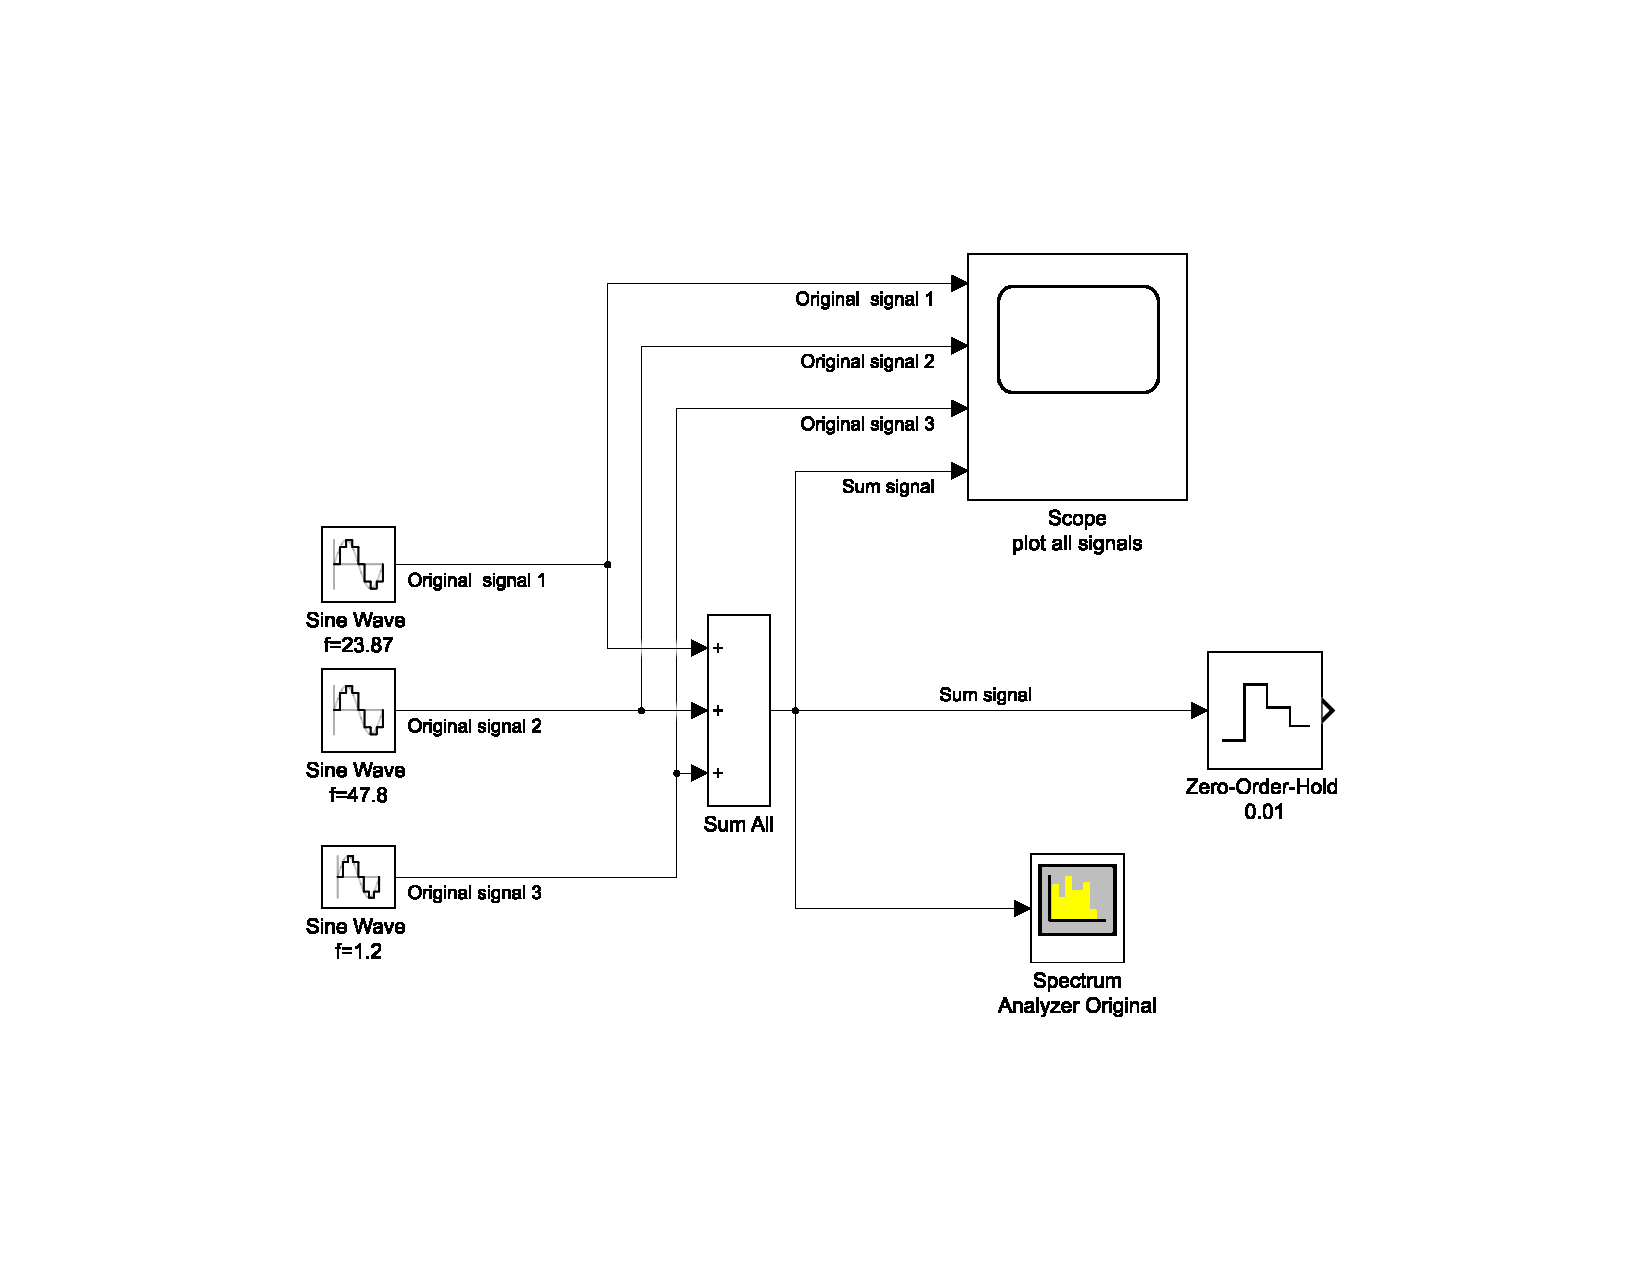
\includegraphics[width=0.7\textwidth]{Bilder/Lauferkennung_Freqbasiert_TestBeispiel_SinussignalGenerator.pdf}
	\caption{Testbeispiel - Frequenzbasierte Lauferkennung - Sinussignal}
	\label{fig:Lauferkennung_Freqbasiert_TestBeispiel_SinussignalGenerator}
\end{figure}

%\begin{figure}[H]
%	\centering
%	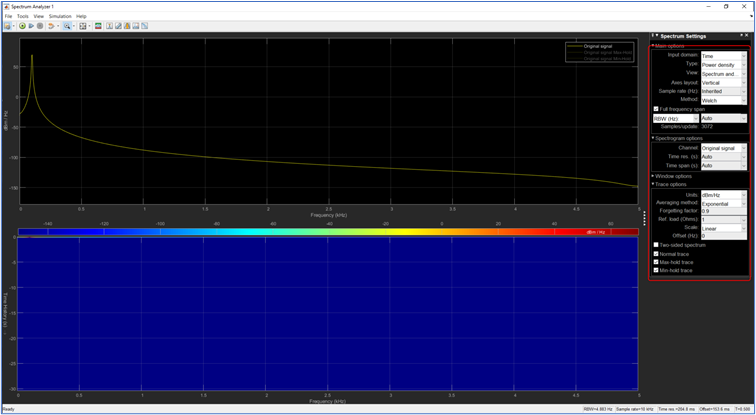
\includegraphics[width=\linewidth]{Bilder/Lauferkennung_Freqbasiert_SpektrumAnalyzerAusgabe.png}
%	\caption{Testbeispiel - Frequenzbasierte Lauferkennung - Ausgabe des Spektrum-Analyzer und seine Spezifikationen}
%	\label{fig:Lauferkennung_Freqbasiert_SpektrumAnalyzerAusgabe}
%\end{figure}

\begin{figure}
	\centering
	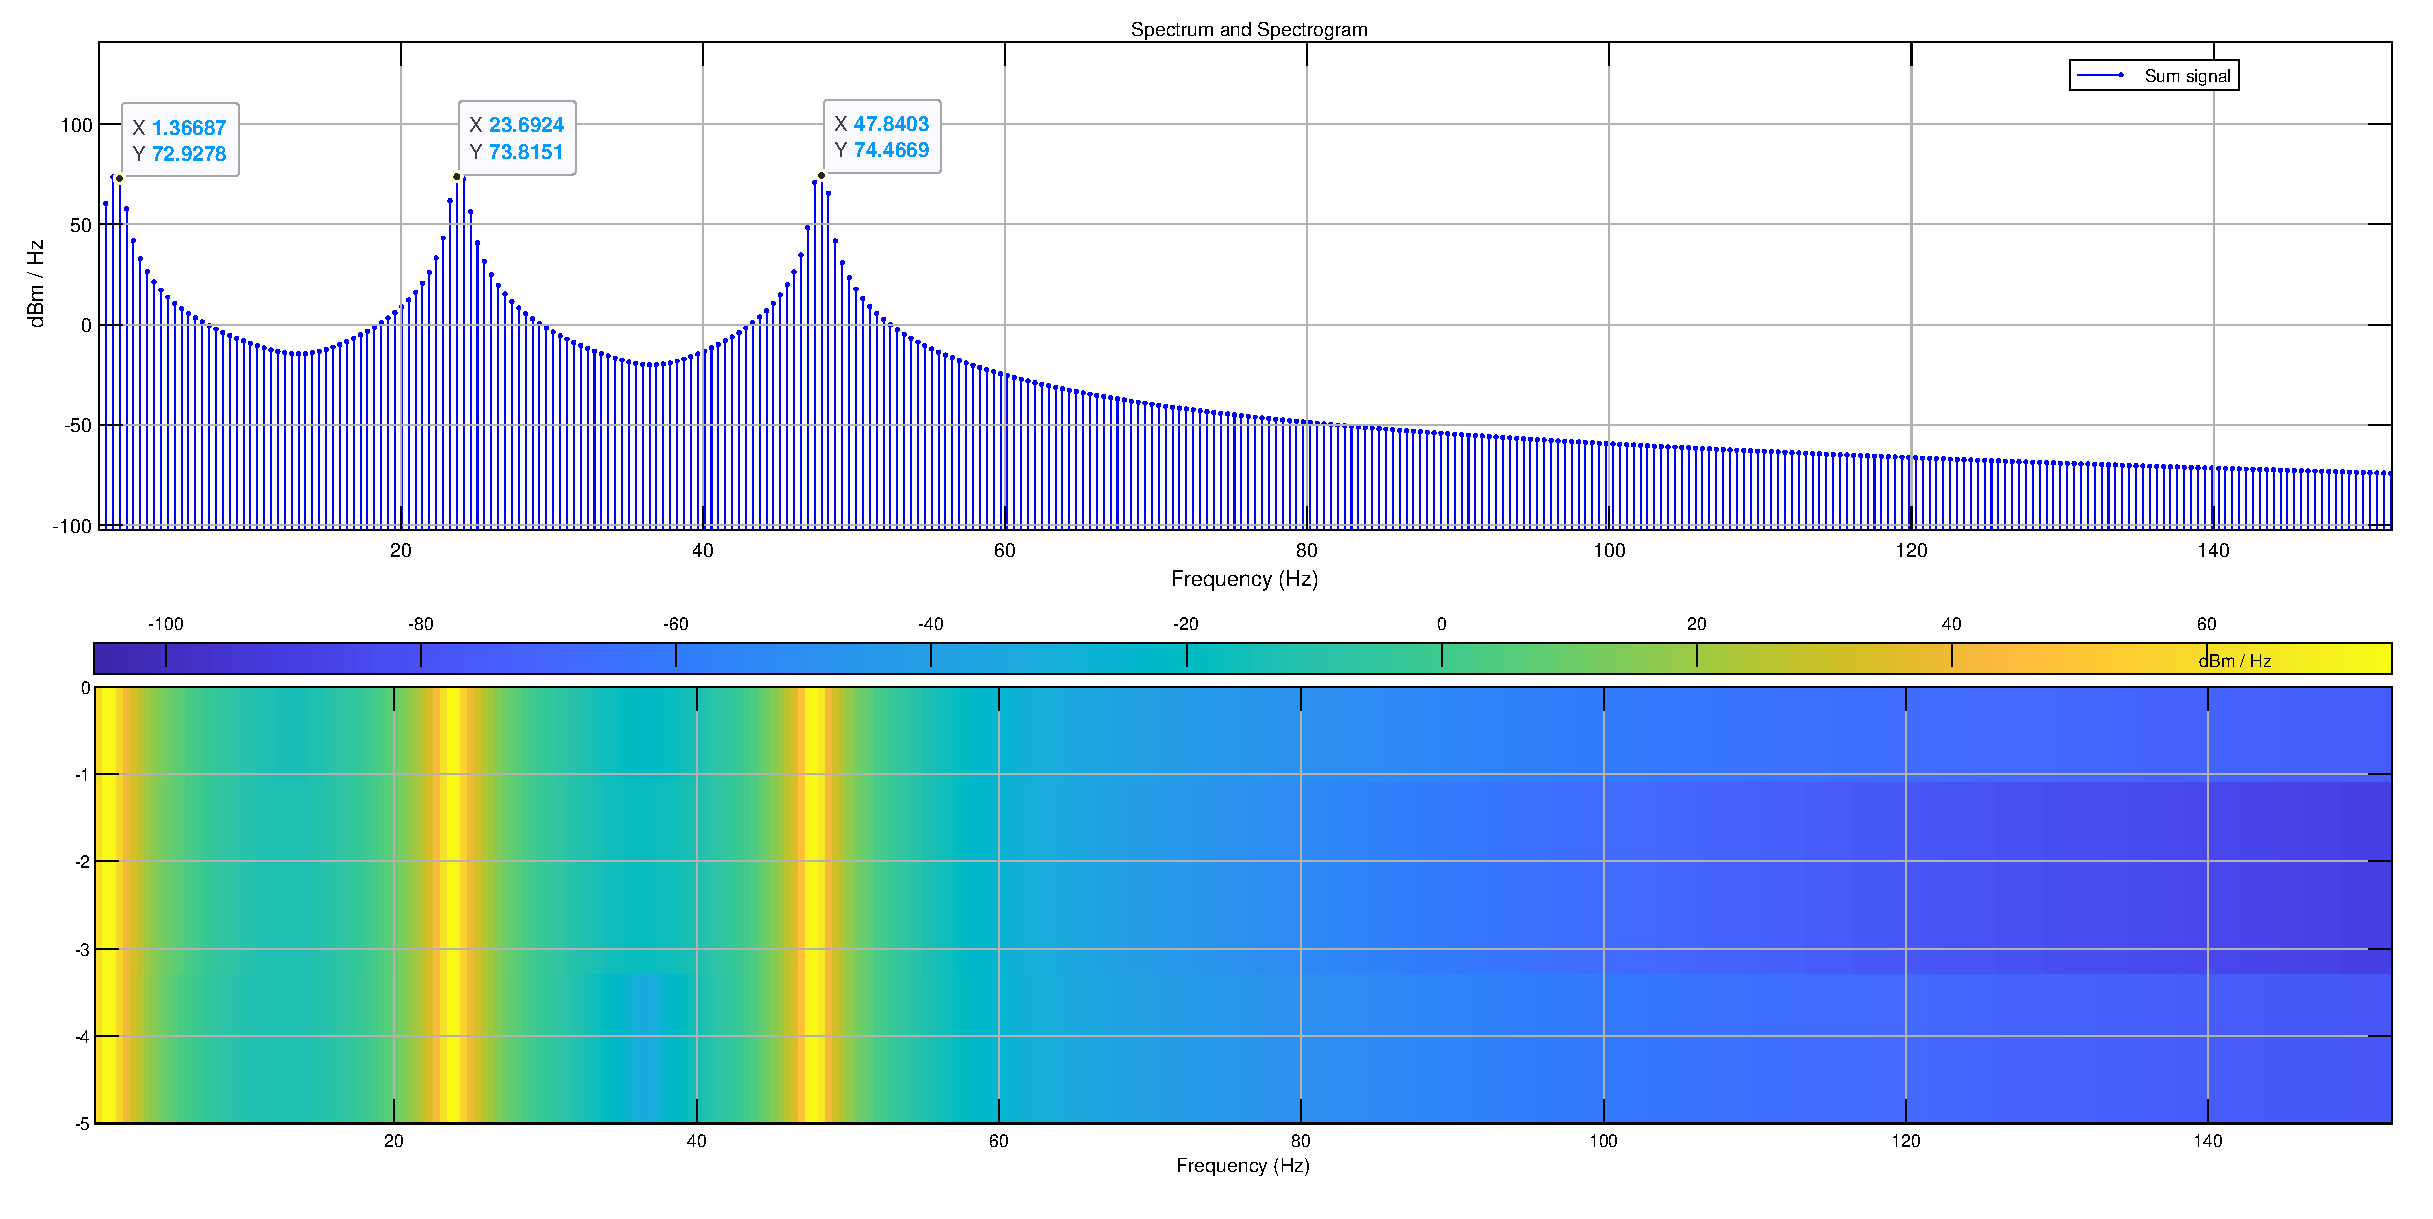
\includegraphics[width=\textwidth]{Bilder/frequenzbasierte_Lauferkennung_SpectrumAnalyzer_Ausgabe2_eps.eps}
	\caption{Testbeispiel - frequenzbasierte Lauferkennung - Ausgabe des Spektrum-Analyzers im Fall eines komplexen Signals}
	\label{fig:Lauferkennung_Freqbasiert_SpektrumAnalyzerAusgabe_gezoomt}
\end{figure}

%Mit anderen Einstellungen in dem Spektrum-Analyzer erhält der Benutzer eine aussagekräftigere Darstellung der Frequenz (siehe \autoref{fig:Lauferkennung_Freqbasiert_SpektrumAnalyzerAusgabe_2Einstellungen})
%
%\begin{figure}[H]
%	\centering
%	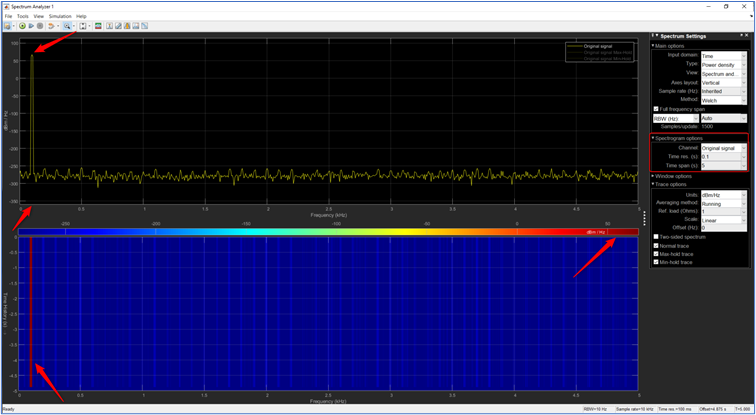
\includegraphics[width=\linewidth]{Bilder/Lauferkennung_Freqbasiert_SpektrumAnalyzerAusgabe_2Einstellungen.png}
%	\caption{Testbeispiel - Frequenzbasierte Lauferkennung - Ausgabe des Spektrum-Analyzer mit anderen Spezifikationen}
%	\label{fig:Lauferkennung_Freqbasiert_SpektrumAnalyzerAusgabe_2Einstellungen}
%\end{figure}

\subsubsection{Testmodel}
Nachdem das gedachte Prenzip getestet wurde, ist nun eine Vervollständigung des Modells wichtig. Das vollständige Testmodel ist in der \autoref{fig:Lauferkennung_Freqbasiert_FFT_Testmodell} veranschaulicht. Das Ziel ist die Funktionalität des Prinzips zu überprüfen, bevor dieses mit einem Echtsignal getestet wird.\\
In dem System sind drei Sinussignale mit verschiedenen Frequenzen generiert, die zusammen summiert werden, um ein komplexes Signal zu erstellen (\autoref{fig:Testsignal_AllViews}).
Eine vereinfachte Ablaufschema des Models ist in der \autoref{fig:Lauferkennung_FFT_Ablaufschema_Testmodell} gezeigt.

Das Testmodel erstellt zuerst ein komplexes Signal mit bekannten Grundfrequenzen und konvertiert dieses mit dem \glqq Zero-Order-Hold\grqq{}-Block zu einem diskreten Signal, da die FFT nicht auf ein kontinuierliches Signal anwendbar ist. Danach wird das FFT-Fenster durch das \glqq Buffer\grqq{}-Block eingestellt und dann die FFT an das entsprechende Fenster angewandt. Das Ergebnis der FFT wird weiterbearbeitet, in dem der Betrag gebildet und die Spiegelung entfernt wird. Das Resultat ist eine 2-D-Matrix mit den Intensitäten sowie ihren Indexe auf die Skala $1$ bis $512$, wobei die Indexe die Frequenzen entsprechen. Das Resultat ist in der \autoref{fig:FFT_Ergebnis_Skala_512} dargestellt. Die Indexe werden extrahiert und in den Skala von 1-100 umgerechnet, in dem diese mit $100/512$ multipliziert.
Das Endergebnis des Models ist eine sortierte Liste der tatsächlichen Grundfrequenzen. Die ersten drei Werte haben eine wesentliche große Intensität und sind somit die gesuchten Frequenzen mit minimaler Abweichung.

\begin{landscape}
	\begin{figure}
		\centering
		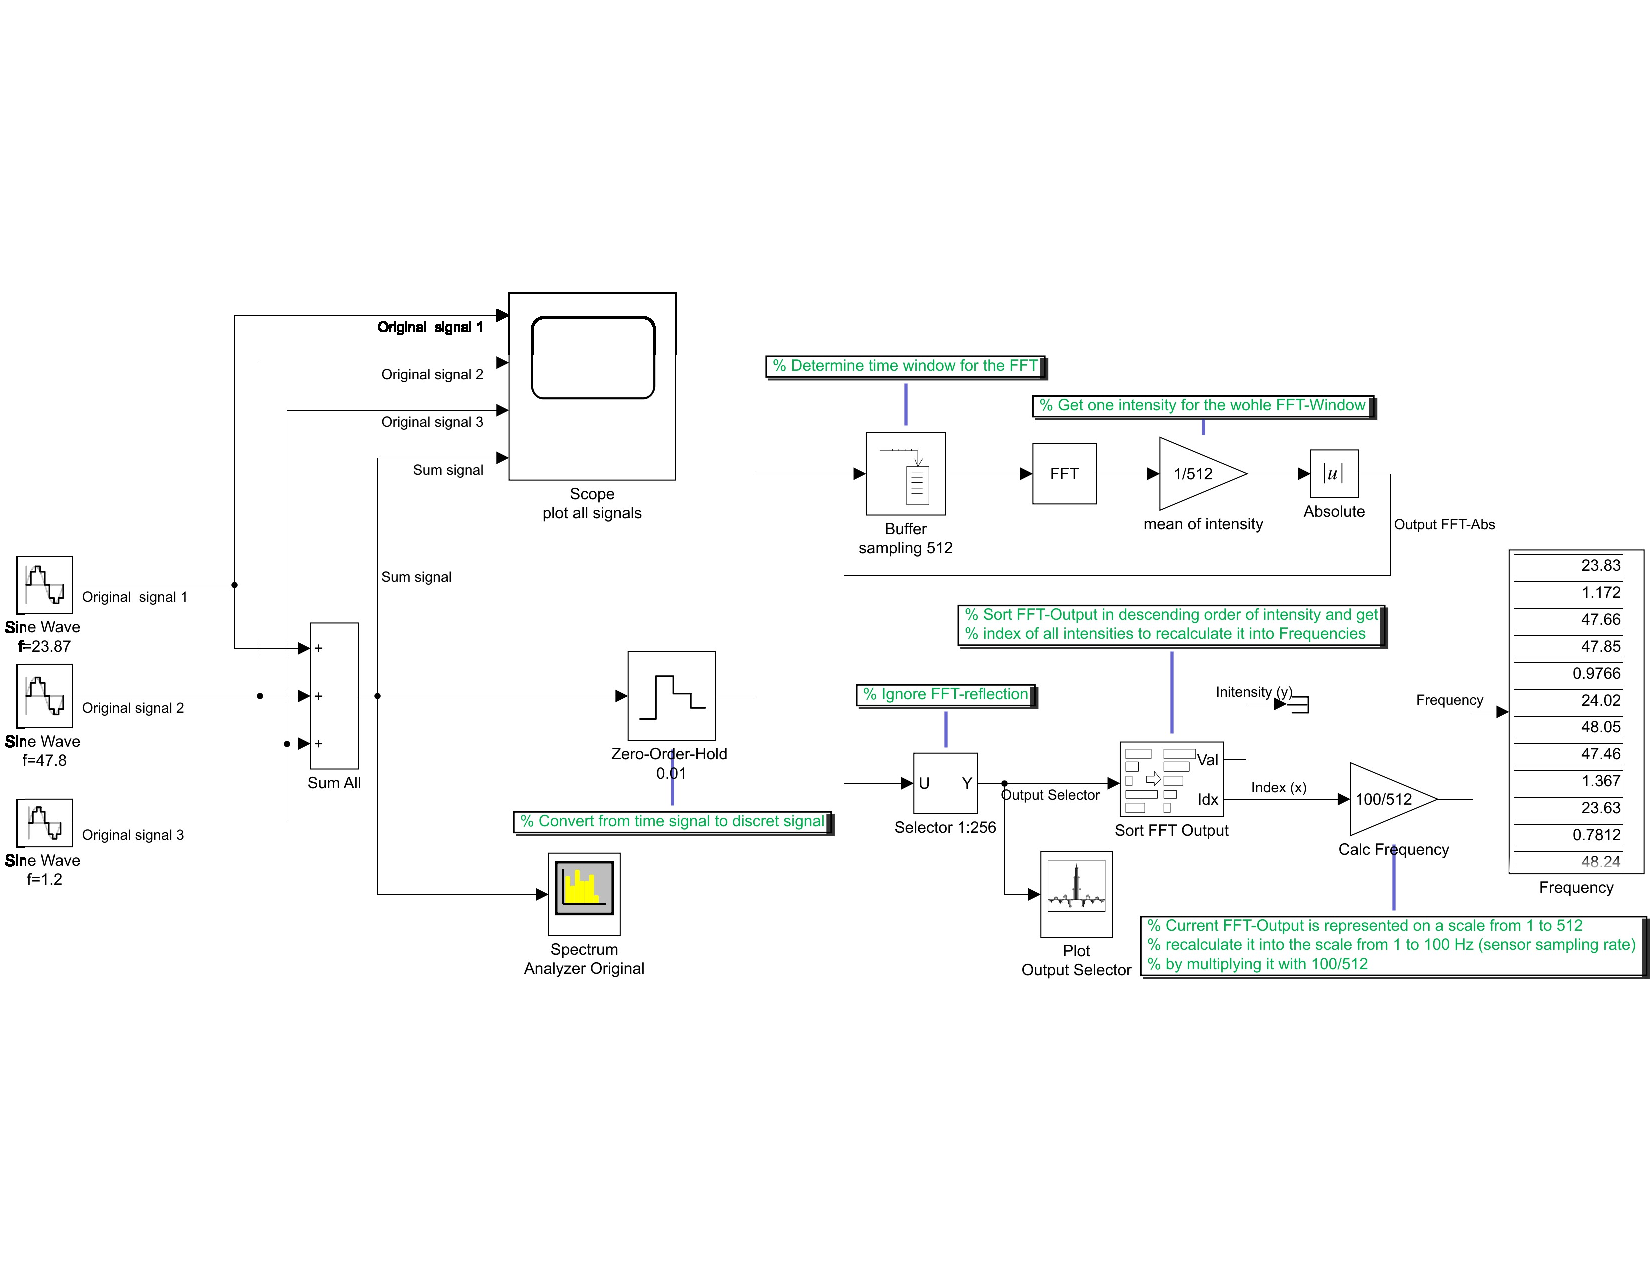
\includegraphics[width=\linewidth]{Bilder/Lauferkennung_FFT_Testmodell1.pdf}
		\caption{Testbeispiel - Frequenzbasierte Lauferkennung - FFT}
		\label{fig:Lauferkennung_Freqbasiert_FFT_Testmodell}
	\end{figure}
\end{landscape}

\begin{figure}
	\centering
	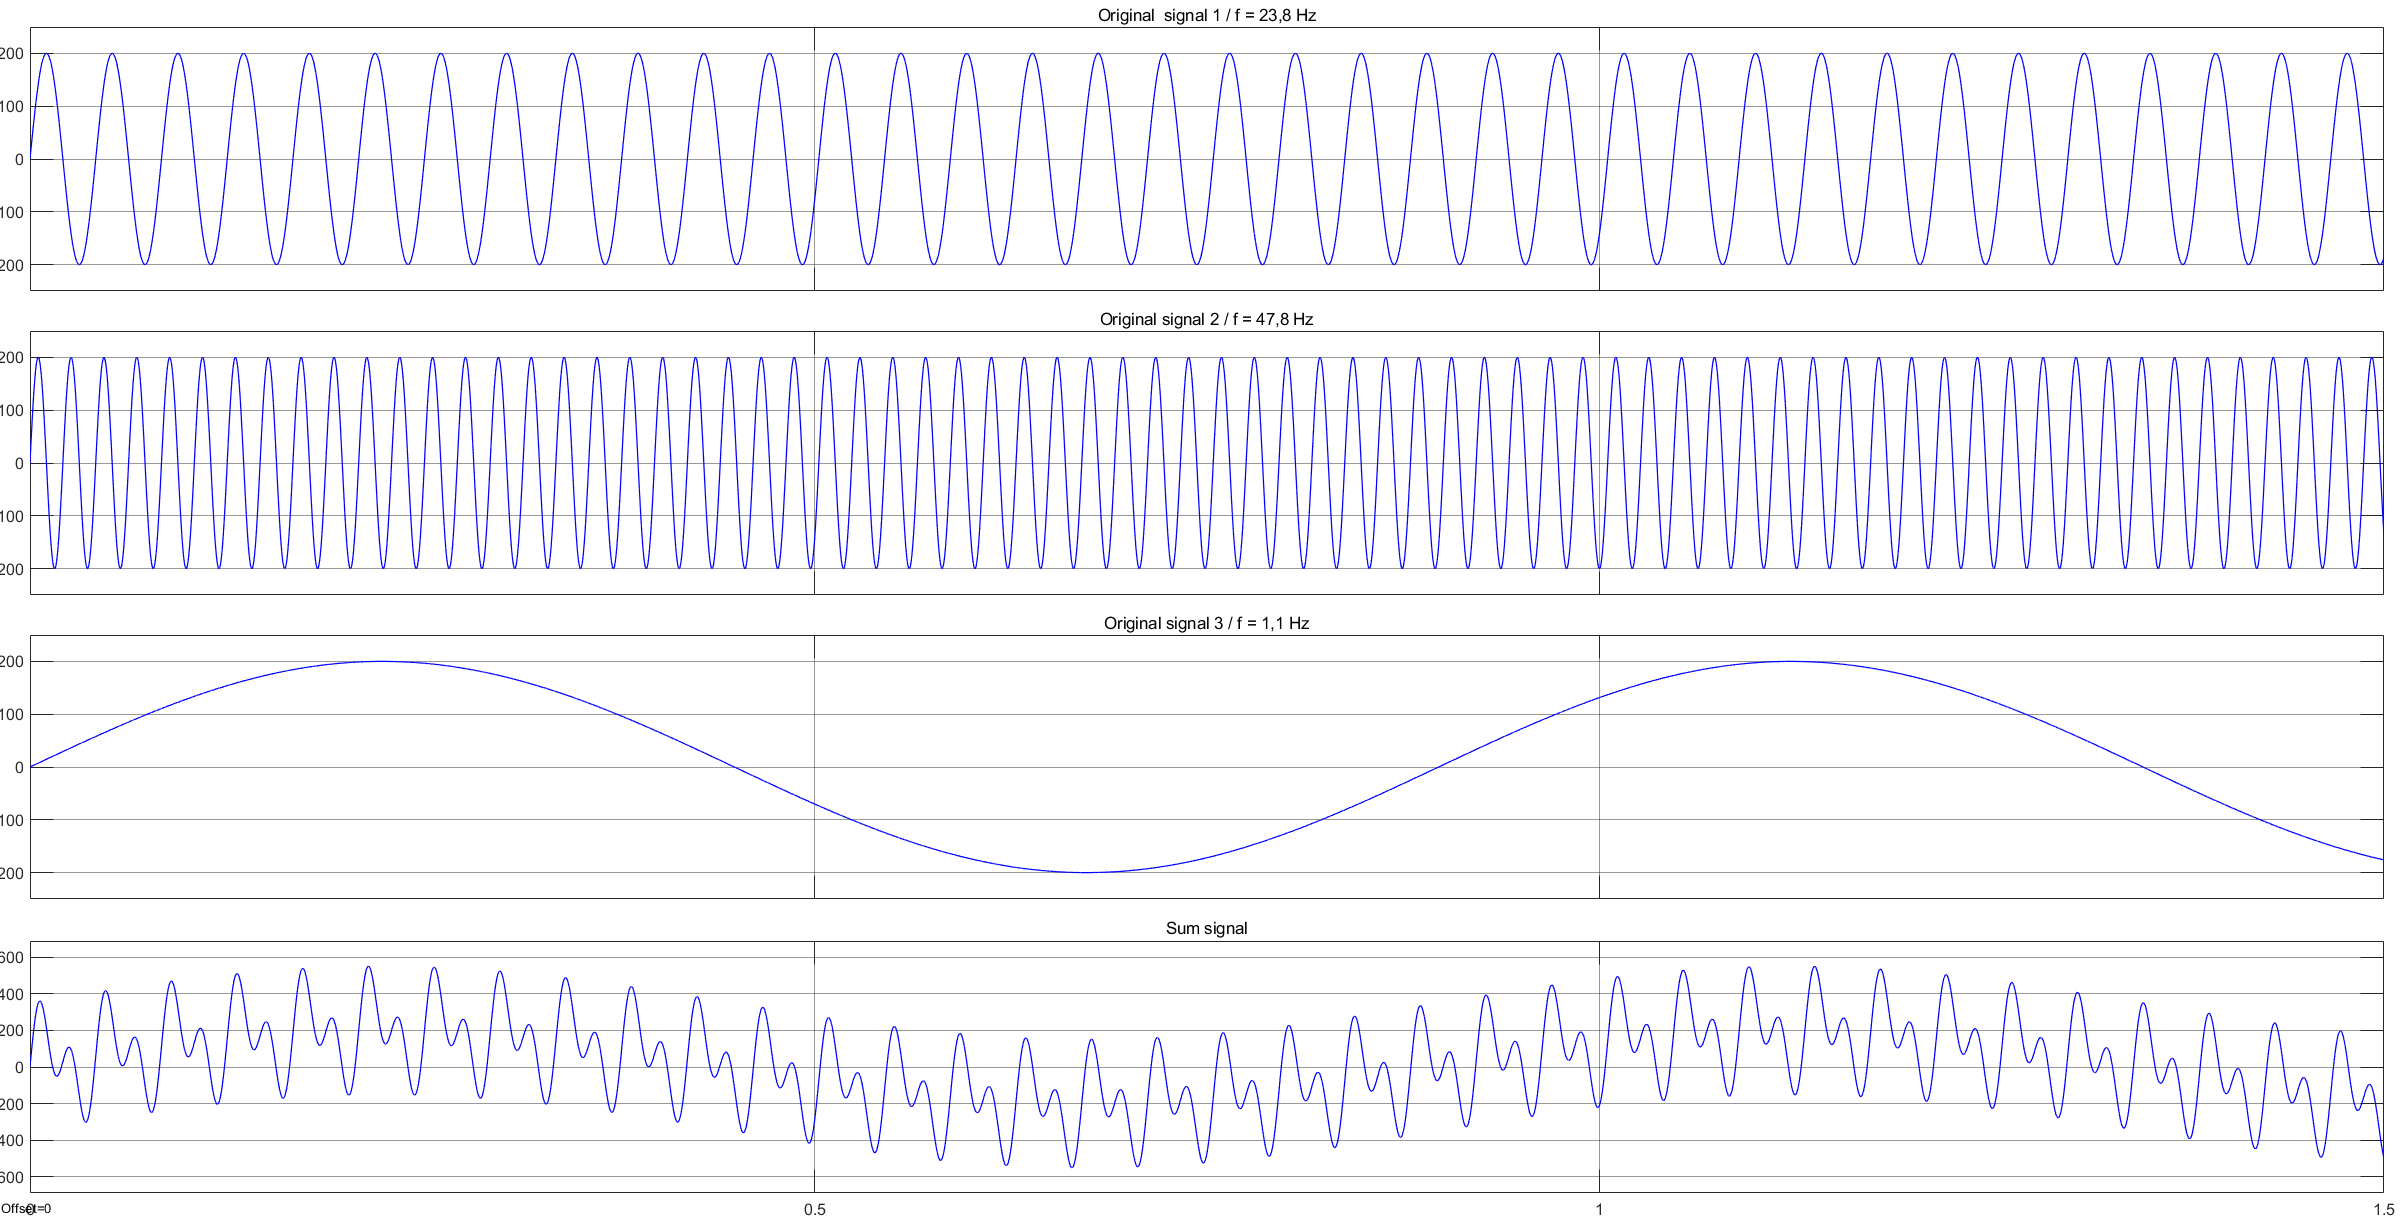
\includegraphics[width=\linewidth]{Bilder/Testsignal_AllViews.png} % TODO: Vektorgrafik
	\caption{verschiedene Einzelsignale ($f=23,8$; $f=47,8$; $f=1,1$) mit deren Summe $f_g$}
	\label{fig:Testsignal_AllViews}
\end{figure}

\begin{figure}
	\centering 
	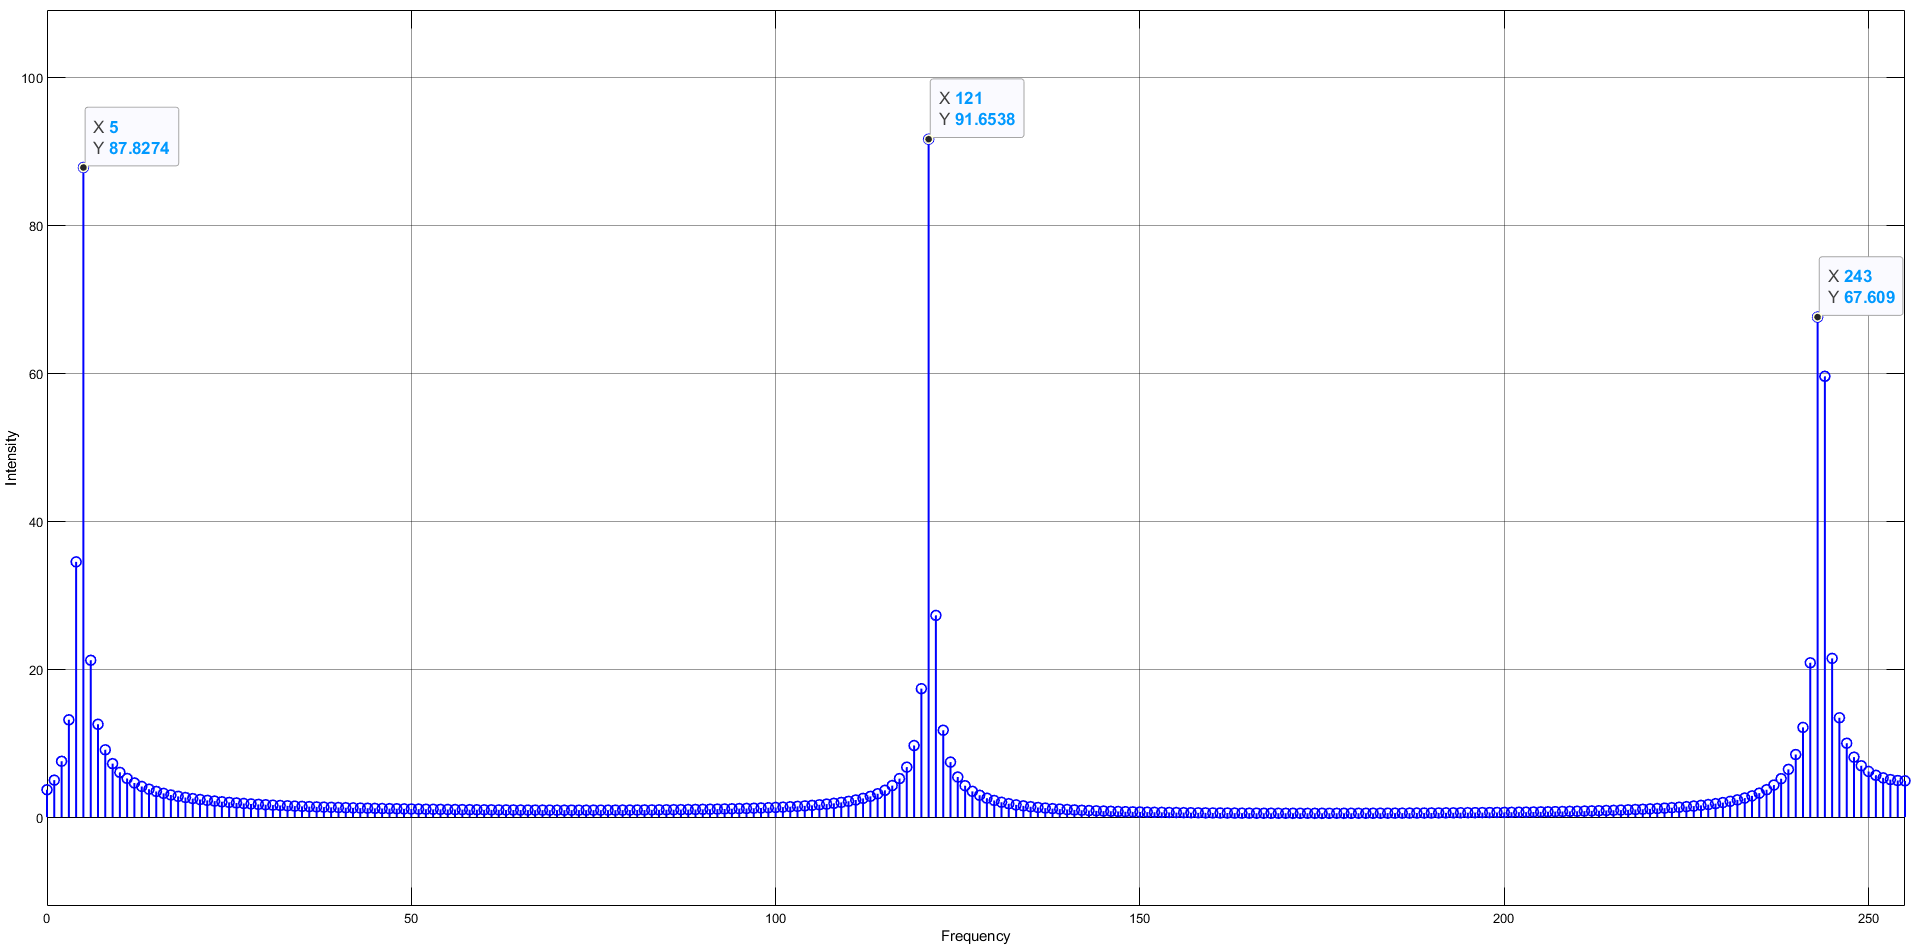
\includegraphics[width=\linewidth]{Bilder/FFT_Ergebnis_Skala_512.png} % TODO: Vektorgrafik
	\caption{Das Ergebnis der FFT - Spiegelung entfernt und Beträge}
	\label{fig:FFT_Ergebnis_Skala_512}
\end{figure}

\begin{figure}
	\centering
	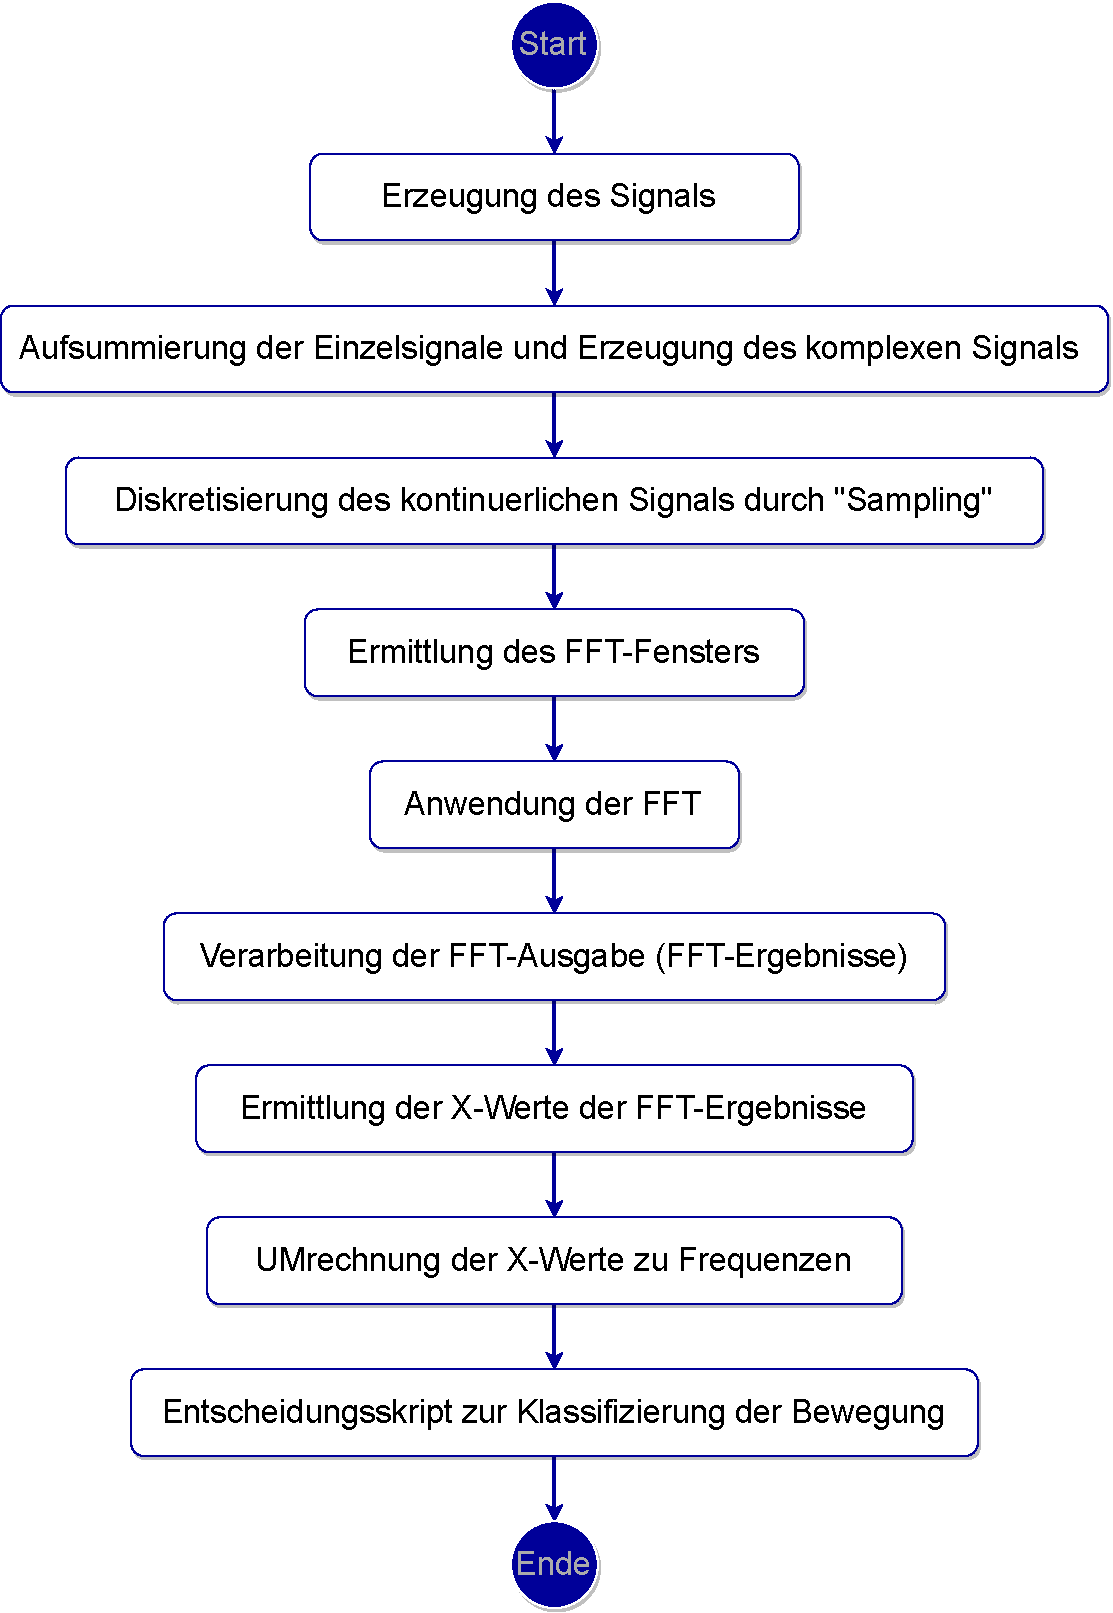
\includegraphics[width=0.7\linewidth]{Bilder/Frequenzermittlung_Ablaufschema_pdf.pdf}
	\caption{Ablaufschema des Testmodels der frequenzbasierten Lauferkennung}
	\label{fig:Lauferkennung_FFT_Ablaufschema_Testmodell}
\end{figure}

Nachdem die Ergebnisse des Testmodels für Richtigkeit geprüft wurden, wird das System mit einem Echtsignal getestet. 

\subsubsection{Anwendung auf ein Echtsignal}

Zum Anwenden auf ein Echtsignal wird ein Untersystem \glqq MotionDetection\grqq{} erstellt, das die Bewegung (Laufen oder fahren) erkennt und zurückgibt.
In der \autoref{fig:Lauferkennung_Freqbasiert_FFT_Echtmodell} ist einen Teil des genannten Models sichtbar. 

Im ersten Teil (1) wird der Betrag aller drei Beschleunigungskomponenten (X,Y,Z) ausgerechnet und dieser für die Lauferkennung verwendet, um diese unabhängig von der Laufrichtung zu bewahren. Der erste Teil kann wie folgt mathematisch beschrieben werden:
\begin{align*}
	Acc_g = \sqrt{ Acc_X^2 + Acc_Y^2 + Acc_Z^2}
\end{align*}

In dem zweiten Teil (2) wird eine FFT durchgeführt, um danach die Frequenzen ermitteln zu können. Das Block \glqq Buffer\grqq{} stellt das FFT-Fenster ($B_L$) ein, in dem eine bestimmte Anzahl der Proben (Messungen) gesammelt wird. In diesem Model wird das Fenster auf $B_L = \SI{2,56}{\second}$ (d.h. \SI{256}{Proben}) mit einer Überlappung von $50\%$ eingestellt. Die minimale erkennbare Frequenz lässt sich durch
\begin{align*}
	f_{min} = \frac{1}{B_L} = \SI{0,3906}{\hertz}
\end{align*}
berechnen (siehe \autoref{abs:FFT}).

Eine größeres FFT-Fenster $B_L$ hätte eine bessere Frequenzermittlung gesichert und würde allerdings zu größeren Rechenaufwand und längeren Rechenzeiten führen. Die Überlappung dient dazu die Frequenzen am FFT-Fensterrand besser zu berücksichtigen. Danach wird die FFT-Spiegelung mit der Funktion \glqq Select\grqq{} vernachlässigt. Der Ausgang dieses Teils ist eine 2-D-Liste auf ein Skala von 1 bis 256, die sortiert werden soll.

Der dritte Teil sortiert die entsprechende Liste nach Intensität. Das Block \glqq Sort FFT Output\grqq{} ergibt die Sortierten Intensitäten sowie deren Indexe aus dem ursprünglichen Matrix. Diese Indexe entsprechen die gesuchten Frequenzen auf die Skala (1-256). Mit einer Umrechnung in die Skala (1-100) lassen sich die tatsächliche Frequenzen berechnen. Die \glqq Select\grqq{}-Blöcke dienen dazu eine Rechenzeit zu verkürzen, in dem nur die Frequenzen mit den zehn größten Intensitäten ausgesucht werden, da nur diese später für die Entscheidung relevant sind.

\begin{figure}
	\centering
	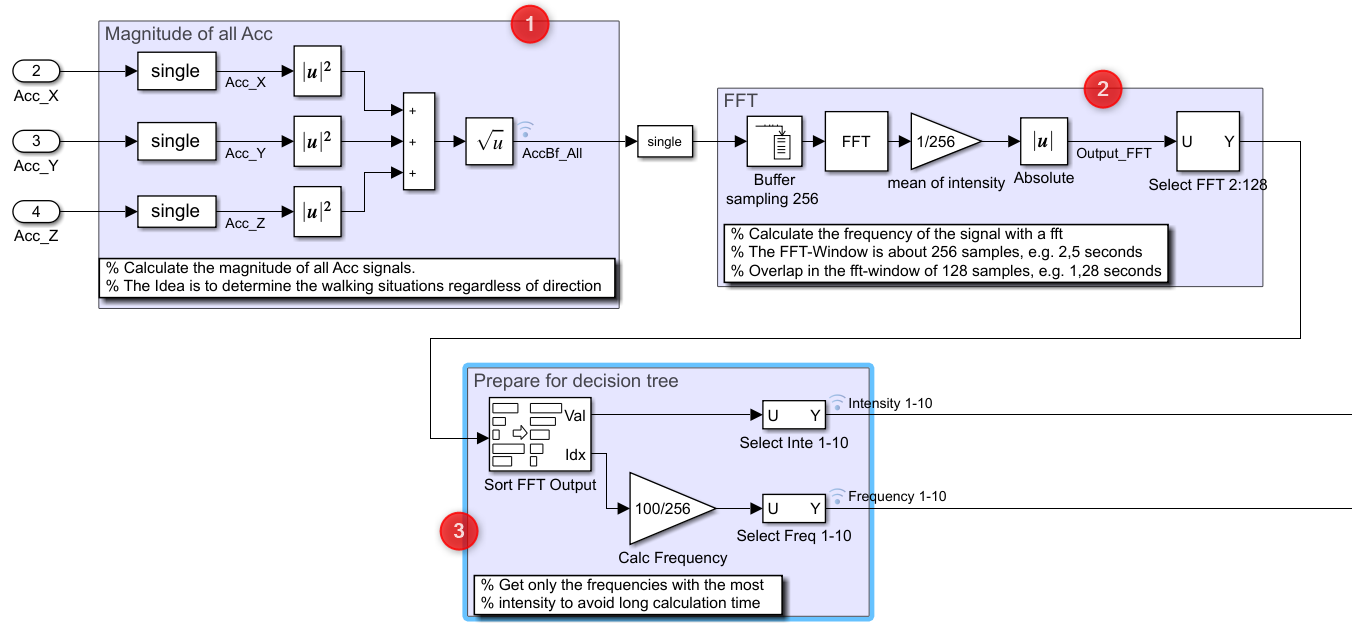
\includegraphics[width=\linewidth]{Bilder/Lauferkennung_Modell_1_1.png}
	\caption{Das vollständige Echtmodel der Frequenzermittlung im Rahmen der Lauferkennung}
	\label{fig:Lauferkennung_Freqbasiert_FFT_Echtmodell}
\end{figure}

Die vom dritten Teil ausgegangenen Daten werden zu einer Matlabdatei (\autoref{fig:getMotionClass_mFile}) geleitet, wo eine Entscheidung getroffen wird.
%
%Die AccBfX, AccBfY und AccBfZ sind die Ausgänge des Modells $CalibrationsMotorbike_V2$ und sie sind die Kalibrierte Signale.
%Diese Werte werden für die Berechnung der Betrag mit der Formel (**********************)
%%TODO: $AccBf_All=√(〖AccBfX〗^2+ 〖AccBfY〗^2+〖AccBfZ〗^2 )$ 
%verwendet (\autoref{fig:Lauferkennung_Freqbasiert_FFT_Spezifikationen})- Nummer 2). Das Ziel ist die Frequenzermittlung richtungsunabhängig zu stellen.
%Danach wurde eine FFT an der Variablen $AccBf_All$ durchgeführt, um die Frequenzen zu ermitteln (\autoref{fig:Lauferkennung_Freqbasiert_FFT}- Nummer 2).
%
%
%\begin{figure}[H]
%	\centering
%	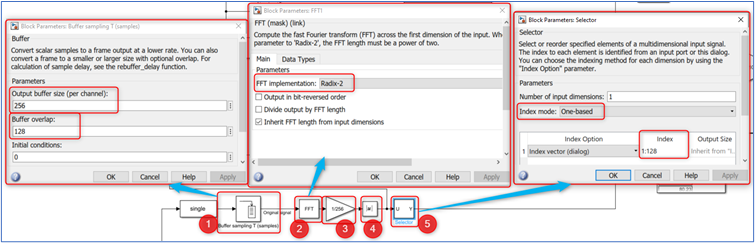
\includegraphics[width=\linewidth]{Bilder/Lauferkennung_Freqbasiert_FFT_Spezifikationen.png}
%	\caption{Testbeispiel - Frequenzbasierte Lauferkennung - FFT - Modell}
%	\label{fig:Lauferkennung_Freqbasiert_FFT_Spezifikationen}
%\end{figure}
%In der \autoref{fig:Lauferkennung_Freqbasiert_FFT_Spezifikationen} wird eine FFT durchgeführt. Die Einstellparameter jedes Element ist ersichtlich.

%1-	In der Buffer sind 256 Samples zu betrachten (d.h. ca. 2,5 Sekunden des Signals, da die Abtastrate der Sensor 100 Hz ist). Eine Überlappung von ca. 1 Sekunde wurde auch eingestellt, damit die Zwischen Frequenzen nicht übersehen werden.\\
%2-	Der FFT-Typ ist eine Radix-2.\\
%3-	Die Ausgabenwerte der FFT durch 265 dividieren. (warum?)\\ %TODO: warum 
%4-	Betrag des FFT-Ausgangs bilden (warum?)\\ %TODO: warum 
%5-	Da FFT ein gespiegelter Ausgang liefert wird nur die Hälfte der Matrix angenommen (1:128)\\
\subsubsection{Entscheidungskriterien - Matlabskript}
%
%
%
%
%
Die \autoref{fig:getMotionClass_mFile} zeigt die Matlab-Funktion, die die Entscheidung übers Laufen treffen soll. Die Eingänge der Funktion sind die zehn Frequenzen mit den höchsten zehn Intensitäten sowie die aktuelle Geschwindigkeit. Die durch die Funktion letzte erkannte Aktivität sowie deren Zeitpunkt werden auch in die Funktion weitergeleitet. Nach dem Durchlauf liefert die Matlab-Funktion eine ID-Zahl, die eine Aktivität entspricht. Der Aktivität-ID-Zusammenhang ist in der \autoref{tab:MotionClass} abgebildet. Das Skript unterscheidet zwischen vier Klassen. Es wird hauptsächlich zwischen Laufen und Fahren unterschieden, sollte diese Entscheidung nicht möglich, liefert das Skript eine Aussage (Unbekannt oder Konflikt) zurück.
Die entscheidende Funktion ist Teil des Simulink-System

\begin{figure}
	\centering
	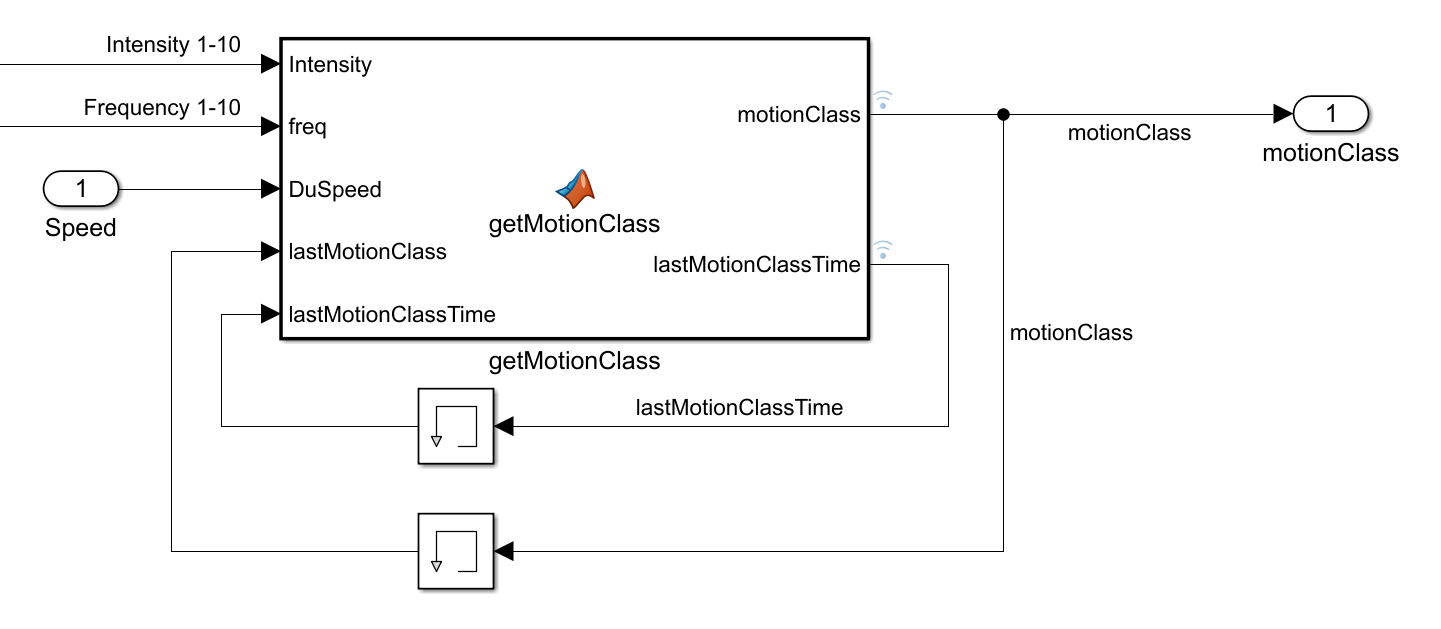
\includegraphics[width=\linewidth]{Bilder/getMotionClass_mFile.png}
	\caption{Ein- und Ausgänge des Entscheidungsskripts}
	\label{fig:getMotionClass_mFile}
\end{figure}

\begin{table}
	\caption{Ausgangsmöglichkeiten der Entscheidungsfunktion} 
	\centering
	\begin{tabular}{|l|l|}%{|p{3.2cm}|>{\centering\arraybackslash}p{3.3cm}|>{\centering\arraybackslash}p{3.3cm}|>{\centering\arraybackslash}p{3.3cm}|}
			\hline
			\textbf{ID} & \textbf{Aktivität} \\
			\hline
			-1 & Konflikt/Fehler \\
			\hline
			0 & Keine Bewegung \\
			\hline
			1 & Laufen \\
			\hline
			2 & Fahren \\
			\hline
		\end{tabular}
	\label{tab:MotionClass}
\end{table}

\begin{figure}
	\centering
	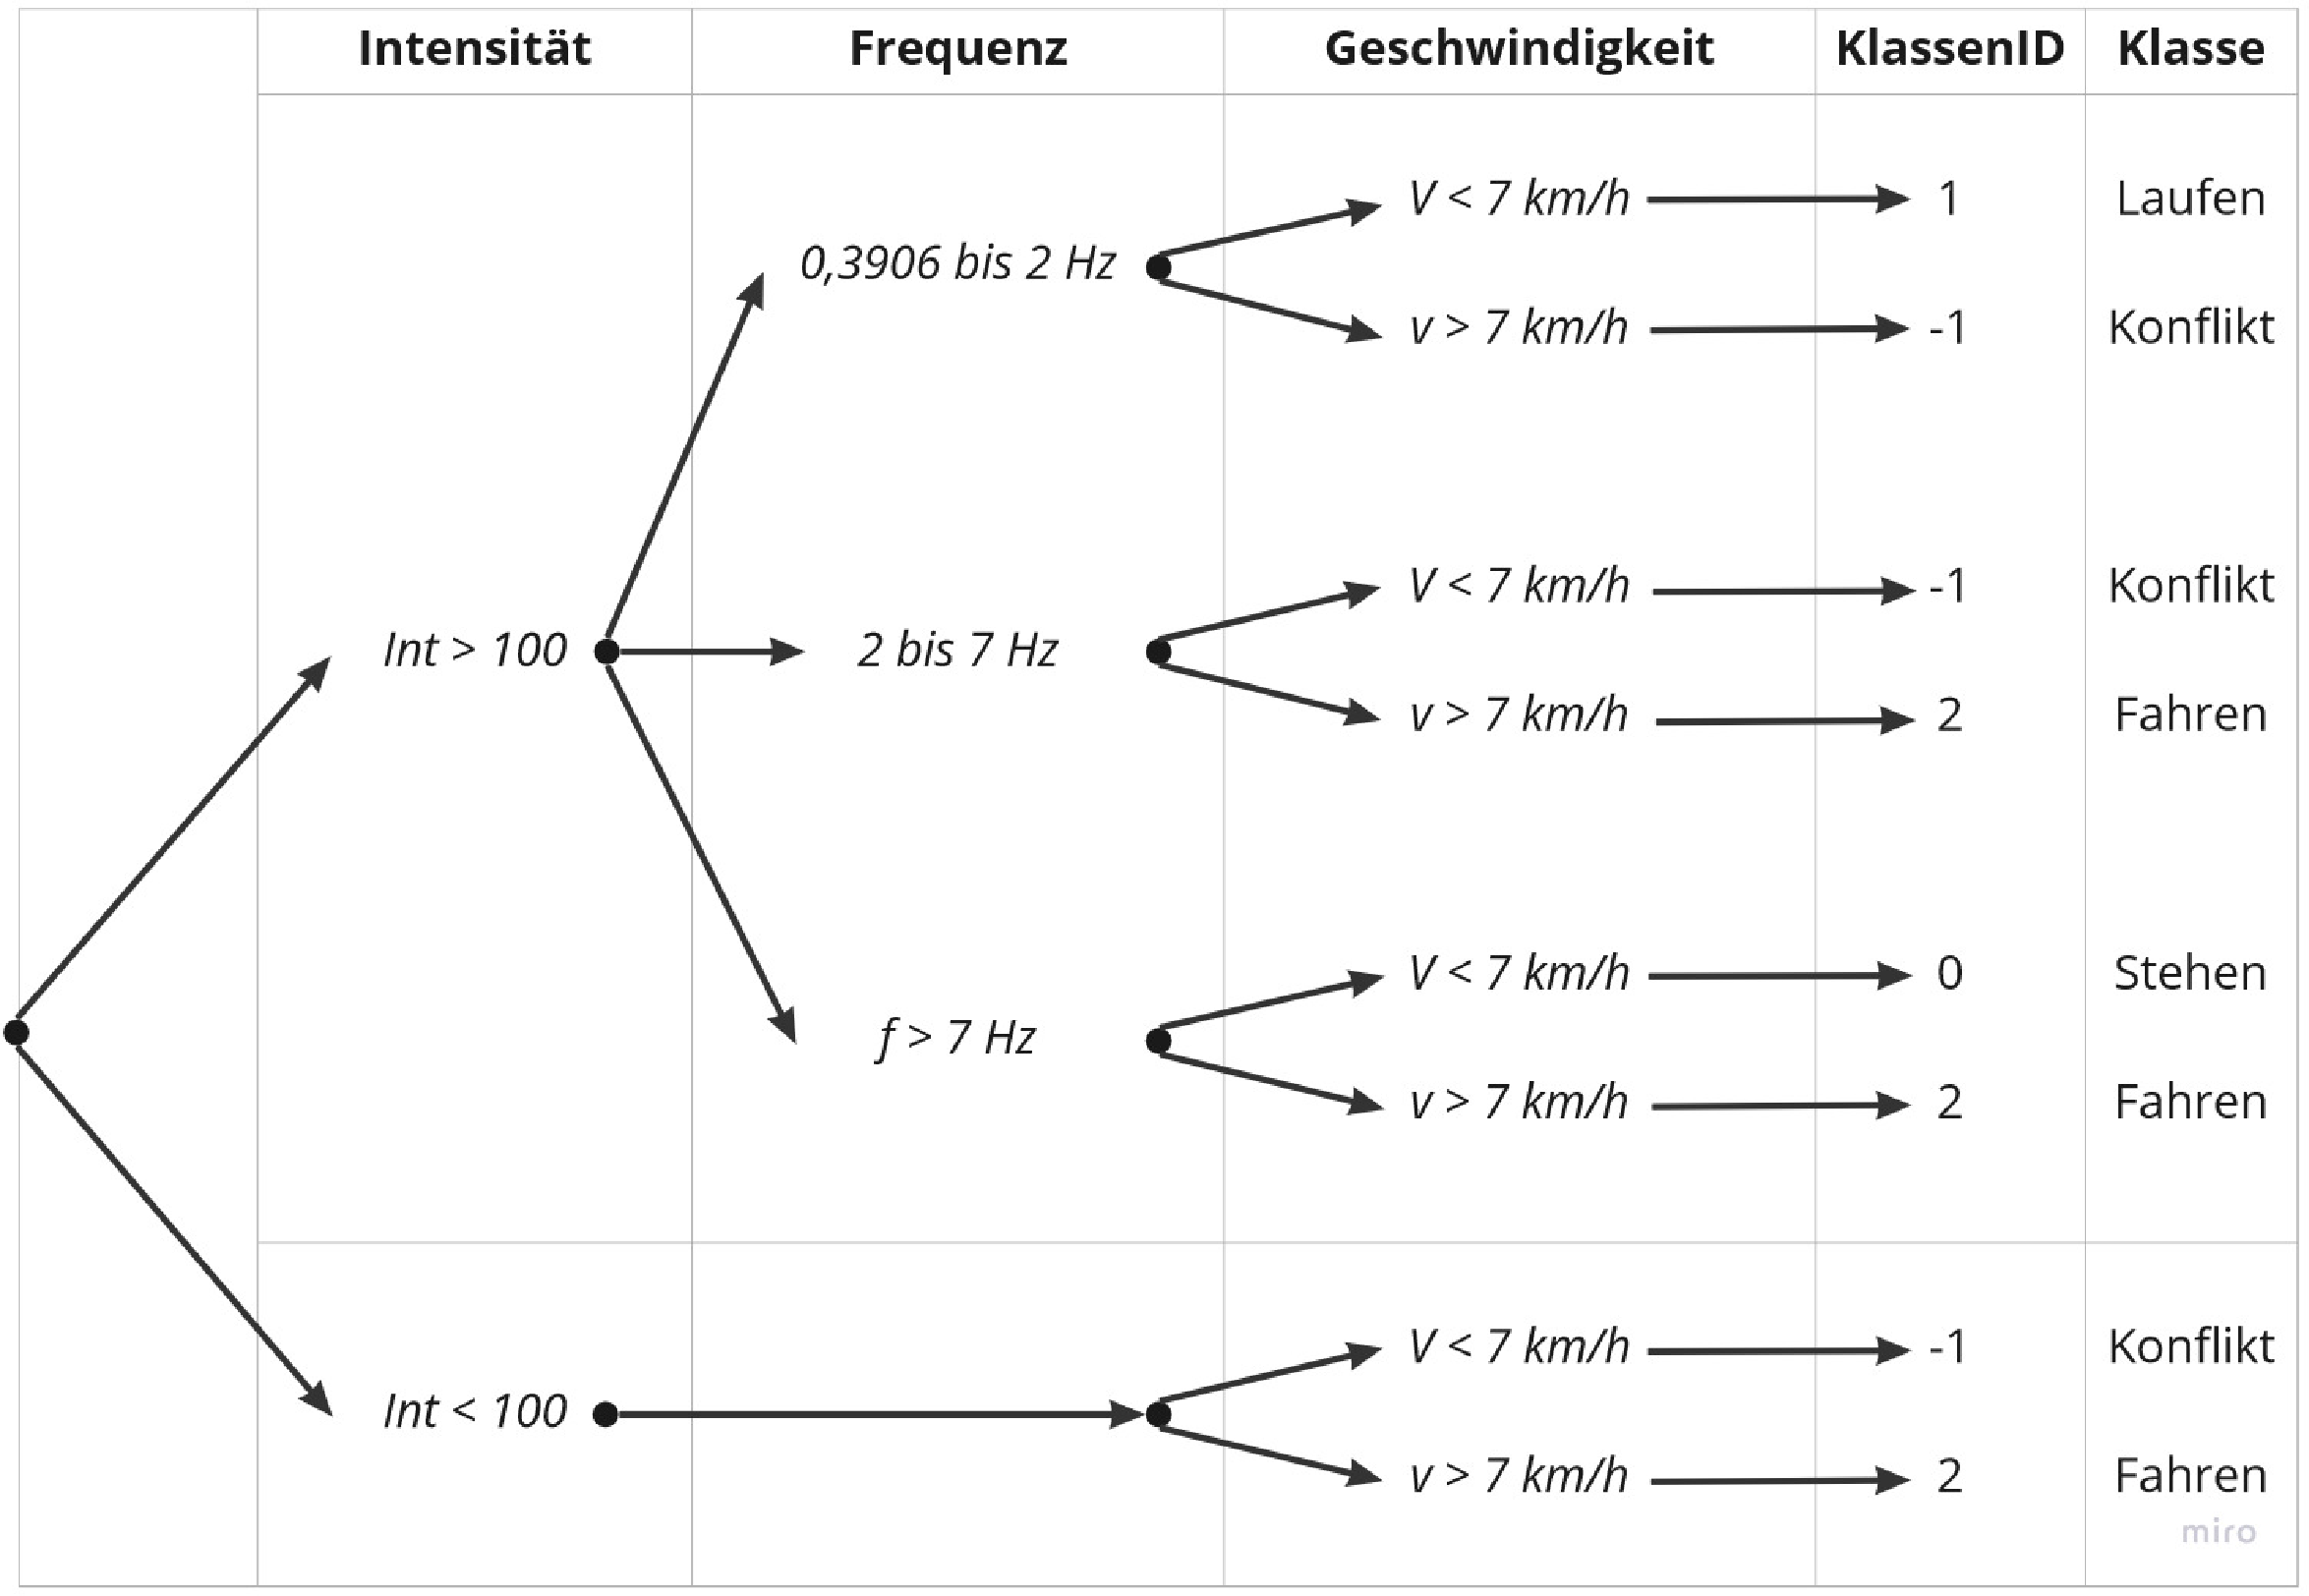
\includegraphics[width=\linewidth]{Bilder/Entscheidungsbaum_mFile.pdf}
	\caption{Entscheidungsbaum der Aktivitätserkennung}
	\label{fig:Lauferkennung_FFT_Entscheidungsbaum_mFile}
\end{figure}

Die \autoref{fig:Lauferkennung_FFT_Entscheidungsbaum_mFile} zeigt das vereinfachte Entscheidungsbaum, wonach die Aktivitäts\-erkennung erfolgt wird.

Die drei Hauptkriterien sind die Frequenz mit ihrer Intensität sowie die gemessene Geschwindigkeit. Wenn die Intensität einen Zulässigen Wert hat, wird die dazugehörige Frequenz berücksichtigt und danach die gelieferte Aussage mit der Geschwindigkeit nachgeprüft.
In dem Entscheidungsbaum sind vier Klassen definiert.
\begin{itemize}
	\item Keine Bewegung
	\item Laufen
	\item Fahren
	\item Konflikt: Wenn die Entscheidungskriterien (Frequenz und Geschwindigkeit) verschiedene Aussagen liefern
\end{itemize}
Der Entscheidungsbaum fängt bei der Intensität an. Wenn die größte Intensität kleiner als der Schwellwert ($100$) ist, kann die dazugehörige Frequenz für die Entscheidung nicht vertrauend sein und werden bis zu vier nachfolgenden Intensitäten untersucht. Sollte immer noch keine zulässige Intensität ergeben, wird sofort nach Geschwindigkeit geschaut und diese für die Entscheidung verwendet.
Z.B. Bei einer Geschwindigkeit von \SI[per-mode = symbol]{30}{\kilo\meter\per\hour} ist von einer Fahr auszugehen und bei \SI[per-mode = symbol]{3}{\kilo\meter\per\hour} vom Laufen.

Kommt eine zulässige Intensität vor, wird die dazugehörige Frequenz berücksichtigt. Eine Frequenz unter \SI{2}{\hertz} bedeutet \glqq Laufen\grqq{} und über \SI{7}{\hertz} entspricht \glqq Fahren\grqq{}. Es wird danach mit der Geschwindigkeit nachgeprüft. Eine Geschwindigkeit von über \SI[per-mode = symbol]{7}{\kilo\meter\per\hour} bedeutet auf jeden Fall \glqq Fahren\grqq{} und darunter \glqq Laufen\grqq{}.
Wenn die Frequenz- und Geschwindigkeitsüberprüfung verschiedene Aussagen zurückgeben, ist von einem Konfliktsituation auszugehen. In diesem Fall werden bis zu vier größten nachfolgenden Frequenzen überprüft.


\subsubsection{Testbeispiel}
Die Signale in der \autoref{fig:AbschnitteBeispielsignal} sind aus einem Echtsignal ausgeschnitten, in dem der Fahrer nach einer Fahrt gelaufen ist. Das Fahren ist in der \autoref{fig:AccZ_Driving_8Sec} sowei das Laufen in der \autoref{fig:AccZ_Walking_8Sec} abgebildet.

Nachdem Aktivitätserkennung mit diesem Signal getestet wurde, hat das Model die richtigen Frequenzen erkannt.
Für das erste Teilsignal aus der \autoref{fig:AccZ_Driving_8Sec} hat eine Frequenz von durchschnittlich \SI{20}{\hertz} geliefert. Das Teilsignal aus der \autoref{fig:AccZ_Walking_8Sec} hat eine Frequenz von etwa \SI{1,8}{\hertz}. Die Frequenzermittlung der Lauferkennung war sehr nah zur Realität.
Nachdem die Frequenzen ermittelt wurden, sind diese ins Entscheidungsskript weiterzuleiten. Das Skript entscheidet dann mit einer Geschwindigkeitsprüfung, welche Aktivität (Fahren oder Laufen) vorgekommen ist.


\begin{figure}
	\centering
	\begin{subfigure}{\textwidth} %TODO: Vektorgrafik
		\centering
		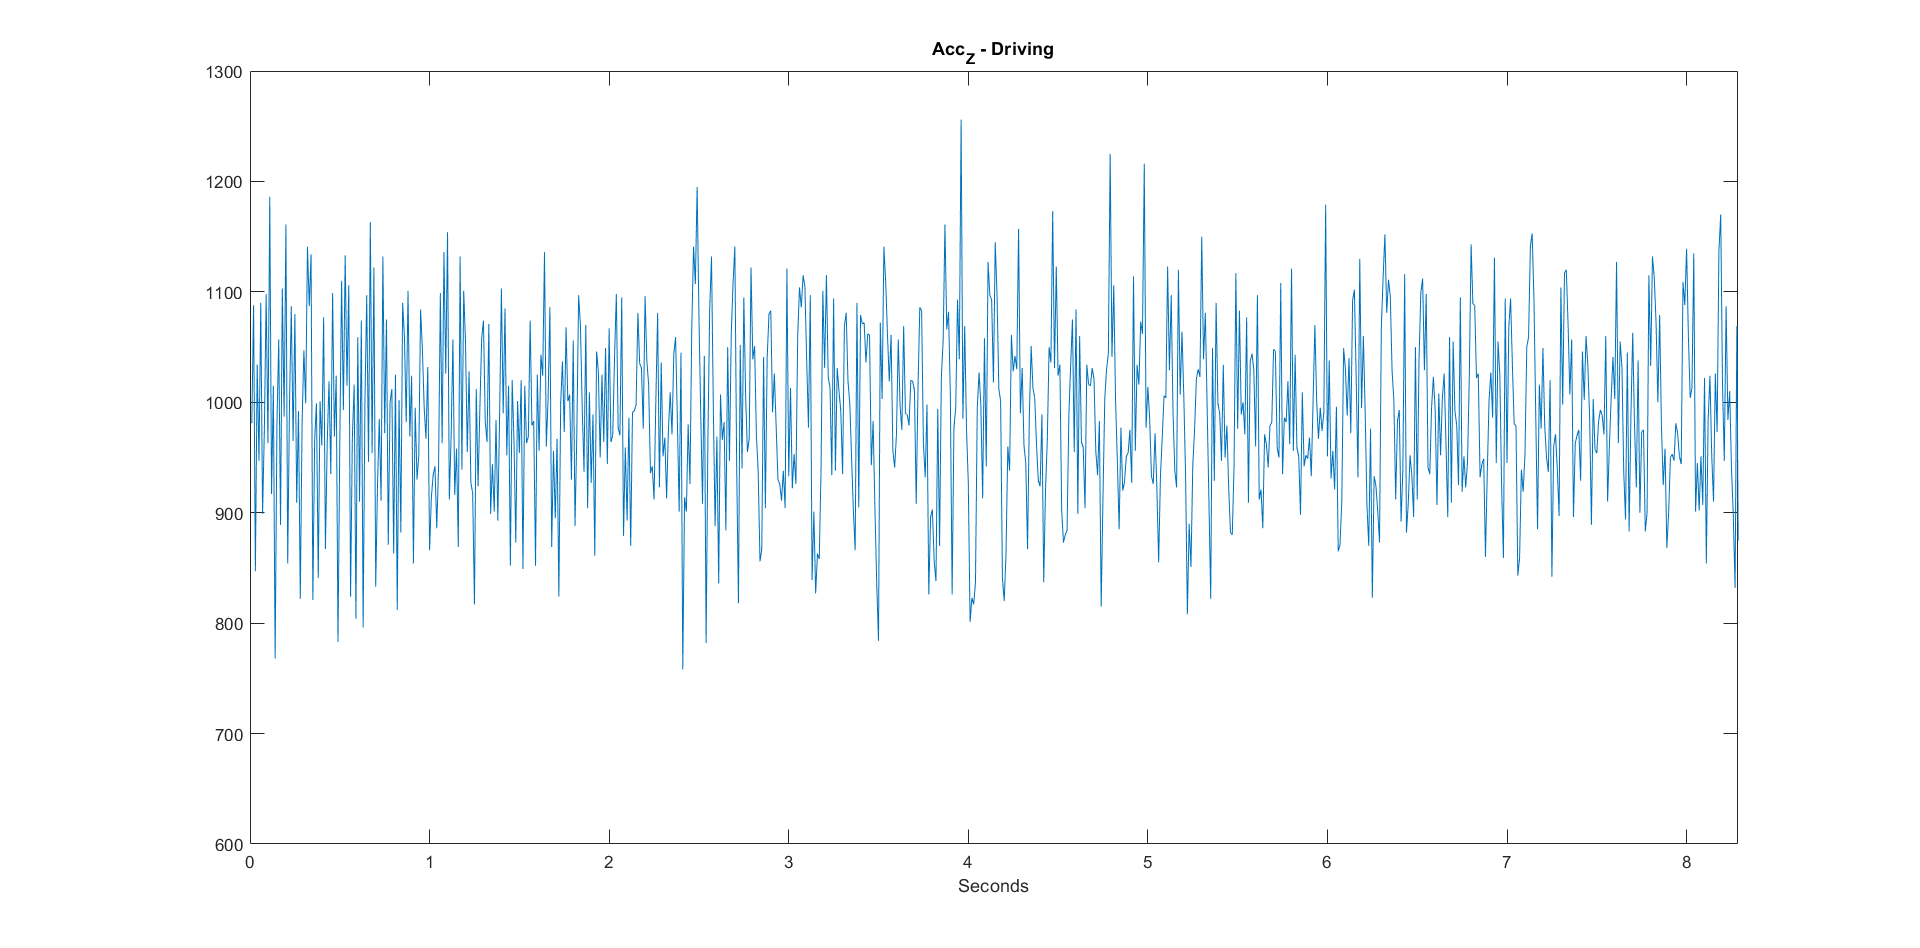
\includegraphics[width=\textwidth]{Bilder/AccZ_Driving_8Sec.png}
		\caption{Beispielsignal - Laufen}
		\label{fig:AccZ_Driving_8Sec}
	\end{subfigure}
	\hfill
	\begin{subfigure}{\textwidth}
		\centering
		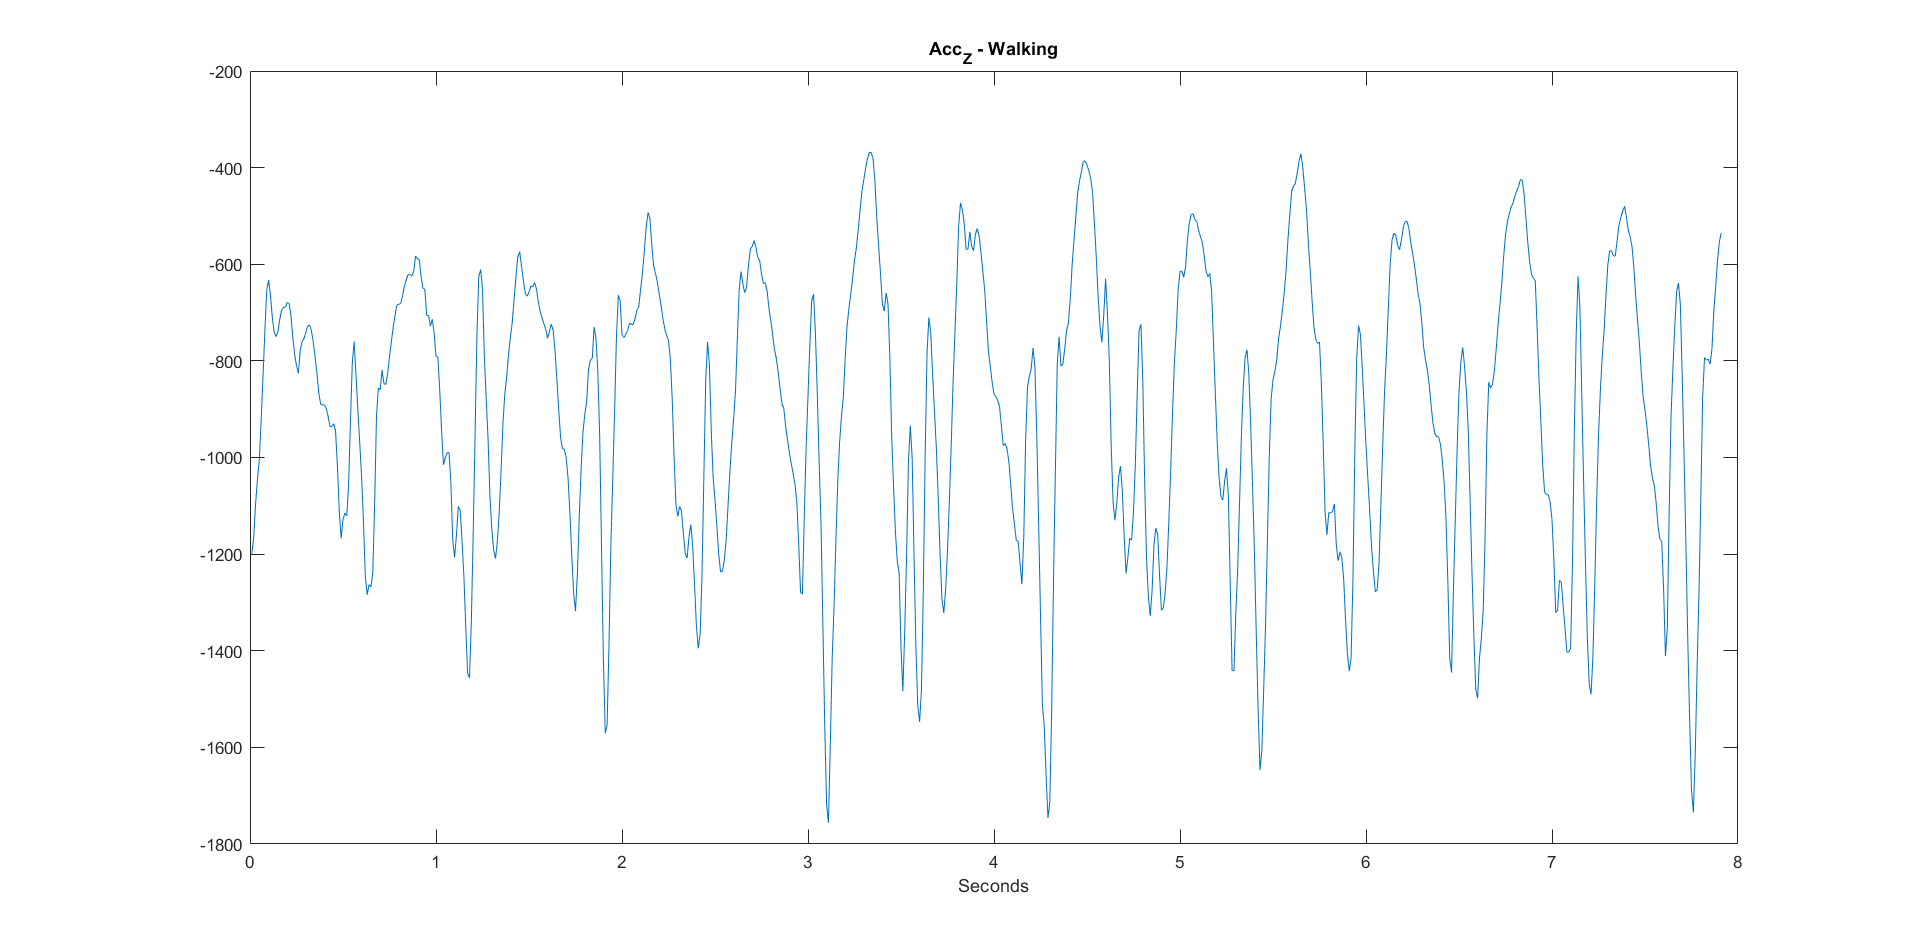
\includegraphics[width=\textwidth]{Bilder/AccZ_Walking_8Sec.png}
		\caption{Beispielsignal - Fahren}
		\label{fig:AccZ_Walking_8Sec}
	\end{subfigure}
	\caption{Abgeschnittene Teile eines Beispielsignals}
	\label{fig:AbschnitteBeispielsignal}
\end{figure}



%Mögliche Konflikte: ID = 2488; CrashNoPSAP;\\
%
%\begin{figure}[H]
%	\centering
%	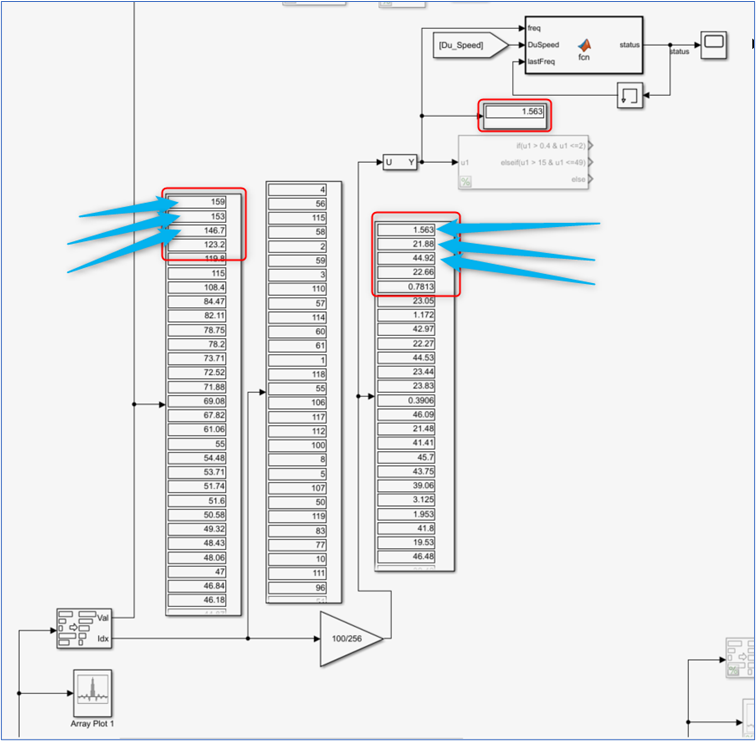
\includegraphics[width=\linewidth]{Bilder/Lauferkennung_Freqbasiert_Ausgangsbeispiel.png}
%	\caption{Testbeispiel - Frequenzbasierte Lauferkennung - Ausgangsbeispiel - ID 2488}
%	\label{fig:Lauferkennung_Freqbasiert_Ausgangsbeispiel_ID2488}
%\end{figure}
%Da hier (\autoref{fig:Lauferkennung_Freqbasiert_Ausgangsbeispiel_ID2488} und \autoref{fig:Lauferkennung_Freqbasiert_Ausgangsbeispiel_ID2488_Scope}) die maximale Intensität der Frequenz 1,5, wird diese als das Maximum übernommen und weiterbearbeitet. Die nächste größte Intensität liegt sehr nah dazu und hat die Frequenz 21,88 Hz, was eigentlich richtiger ist.
%
%\begin{figure}[H]
%	\centering
%	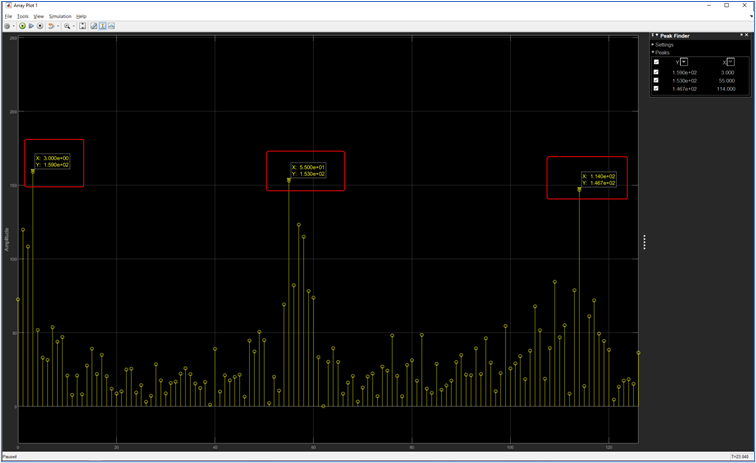
\includegraphics[width=\linewidth]{Bilder/Lauferkennung_Freqbasiert_Ausgangsbeispiel_ID2488_Scope.png}
%	\caption{Testbeispiel - Frequenzbasierte Lauferkennung - Ausgangsbeispiel - ID 2488 - Scope}
%	\label{fig:Lauferkennung_Freqbasiert_Ausgangsbeispiel_ID2488_Scope}
%\end{figure}




\subsubsection{Sinnvolle Werte auswählen}
Nachdem das Testmodel gute Ergebnisse geliefert hatte, sollen die ausgewählte Schwellwerte diskutiert werden.
\begin{itemize}
	\item \textbf{Intensität:} Der Entscheidungsbaum sucht nach einer Intensität von über 100, damit die dazugehörige Frequenz vertrauend zur Entscheidung verwendet werden kann. Nach mehreren Testungen wurde eine Intensität von 100 ausgewählt. Ein niedriger Intensitätswert führt zu einer möglichen falschen Entscheidung, da die Rauschen beziehungsweise die kleinen Frequenzen aus dem Frequenzbereich fälschlicherweise in das Entscheidungsskript eingeleitet werden.
	\item \textbf{Frequenzbereich:} das entspricht der Frequenzbereiche vom Laufen und vom Fahren.\\
	Der Lauffrequenzbereich beträgt in der Regel kleiner als \SI{2}{\hertz}. Das Motorrad schafft wesentlich mehr als \SI{7}{\hertz} (mehr als \SI{420}{Umdrehungen pro Minuten}). 
	\item \textbf{Geschwindigkeit:} In dem Skript ist ein Wert von \SI[per-mode = symbol]{7}{\kilo\meter\per\hour} als Schwellwert zwischen Fahren und Laufen ausgewählt. Der Wert ist in der Straßenverkehrsordnung als Schrittgeschwindigkeit anerkannt\citep{Bussgeldkataloge2022}. Erfahrungsmäßig läuft der Mensch allerdings in einer Geschwindigkeit zwischen \SI[per-mode = symbol]{5}{\kilo\meter\per\hour} und \SI[per-mode = symbol]{10}{\kilo\meter\per\hour}.
\end{itemize}



\section{Auf- und Absteigen} \label{sec:AufAbsteigen}
In der Umgangsphase zwischen Fahren und Laufen steigt die Person ab oder auf. Beim Auf- und Absteigen entsteht eine starke Winkeländerung in der Beinposition, da der Fahrer sein Bein über das Motorrad abhebt und manchmal nach hinten streckt. Wenn das Smartphone in der Hosentasche ist, bekommt es die Winkeländerung ganz klar mit.
Eine theoretische Betrachtung dieser Bewegung schlägt einen Fehlalarmauslösung vor, da die Winkeländerung zu der Sitzposition über \ang{45} liegt, was in der Regel durch das Model \glqq TipOver\grqq{} als Umkippen erkannt wird.
Aus diesem Grund wird dieses Szenario für die Richtigkeit getestet.

%Auch wenn die Winkeländerung den Schwellwert nicht überschreitet, besteht eine hohe Wahrscheinlichkeit, eine Alarmauslösung zu geben, wenn e


%Beim Auf- und Absteigen gibt's starke Winkeländerung im Raum (3D). Wenn einen GH erkannt wird, sollte einen Alarmauslösung ergeben. Ohne GH sollte der Fall nicht als Unfall erkannt.



\section{Anhalten} \label{sec:AmpelStehen}
In diesem Abschnitt wird ein Szenario aus der Tabelle (\autoref{tab:EdgeCasesExcel}) analysiert, in dem der Fahrer während einer Fahrt an eine Ampel für kurze Zeit anhält und sein Fuß runter setzt. In diesem Fall ist das Smartphone in der Hosentasche des bewegenden Beins platziert.
Die Annahme, dass in so einem Fall im Pocket-Mode ein falscher Alarm ausgelöst werden könnte. Der Grund ist die Winkeländerung von ca. \ang{90} zwischen den zwei Beinpositionen, was das Model \glqq TipOver\grqq{} aktiviert und zu einer Alarmauslösung führt.
Die erste Position ist das Bein während einer Fahrt mit der horizontalen Beinstellung. Wenn der Fuß am Boden ist, steht das Bein in einer vertikalen Postion.

In der \autoref{fig:SignalHorizontalUndVertikal} ist ein Beispielsignal eines Smartphones abgebildet. Die Grafik stellt das Signal in zwei Smartphone-Positionen (Vertikal und Horizontal) dar und zeigt einen Winkelunterschied von ca. \ang{90}. Diese Winkeländerung soll das \glqq TipOver\grqq{}-Model aktivieren und schlägt eine Unfallerkennung vor.
Dieses Szenario wird ebenfalls für die Richtigkeit getestet und analysiert.

\begin{figure}
	\centering
	\psfragfig[width=\textwidth]{Bilder/0B_Anglechanging_SmartphonePositions}
	\caption{Winkeländerung im Signal zwischen vertikaler sowie horizontaler Smartphone-Positionierung}
	\label{fig:SignalHorizontalUndVertikal}
\end{figure}



\section{Verifikation des Algorithmus}
Die Verifizierung dient dazu, die Annahmen und Hypothesen aus den letzten Abschnitten zu prüfen, sowie die implementierte Aktivitätserkennung zu testen.


Im Rahmen dieser Verifizierung wird eine Versuchsplanung durchgeführt. Demnächst wird die Versuchsplanung sowie das Versuchsvorgehen erläutert.
%
%
%
\subsection{Versuchsplanung} \label{ab:Versuchsplanung}

In diesem Abschnitt wird auf die zu testenden Szenarien sowie deren Durchführung eingegangen.

Die \autoref{tab:EdgeCasesExcel} zeigt eine Liste der Use- und Edgecases, in der einige Szenarien getestet werden sollen. Es wurden diesbezüglich fünf verschiedene Szenarien geplant.
Die Tabelle (\autoref{tab:TestSzenarienZusammenfassung}) fasst diese zusammen und zeigt die verwendeten Smartphones sowie ihren Ablageorten (Hosentasche, Brusttasche... usw.) während des Testens. Das erste Szenario soll die implementierte Lauferkennung testen sowie das Verhalten beim Auf- und Absteigen aufzeichnen. Dadurch soll das Signalunterschied zwischen der Fahrt und des Laufens erkennbar sein.
Zusätzlich wird die Winkeländerung zwischen der zwei Fahrerpositionen (stehend/sitzend) während einer Fahrt analysiert und getestet.
Das zweite Szenario testet die tatsächliche Winkeländerung zur ursprünglichen Position des Smartphones nach der Kalibrierung sowie die Reaktion des Algorithmus beim Anhalten, da der Fall während einer Fahrt sehr oft vorkommen könnte.

Die dritte sowie vierte Szenario sollen das Verhalten des Smartphones testen, wenn es sich im Tankrucksack ohne Befestigung befindet.
Das letzte Szenario testet die Reaktion des Algorithmus, wenn der Fahrer während einer Fahrt runter fällt und ob der Algorithmus diesen Fall zuverlässig erkennt.
Um die zufällige Fehler bei der Signalaufnahme zu vermeiden werden bei der Testung immer mehr als ein Smartphone verwendet.
Es werden ebenfalls bei manchen Szenarien mehrere Smartphones an mehreren Ablageorten hingebracht, um möglichst viele Daten gleichzeitig zu sammeln und der Verhaltensunterschied des Algorithmus an unterschiedlichen Orten zu forschen.
Die Auswertung dieser Daten wird je nach der verfügbaren Zeit erfolgt.

%\begin{figure}
%	\centering
%	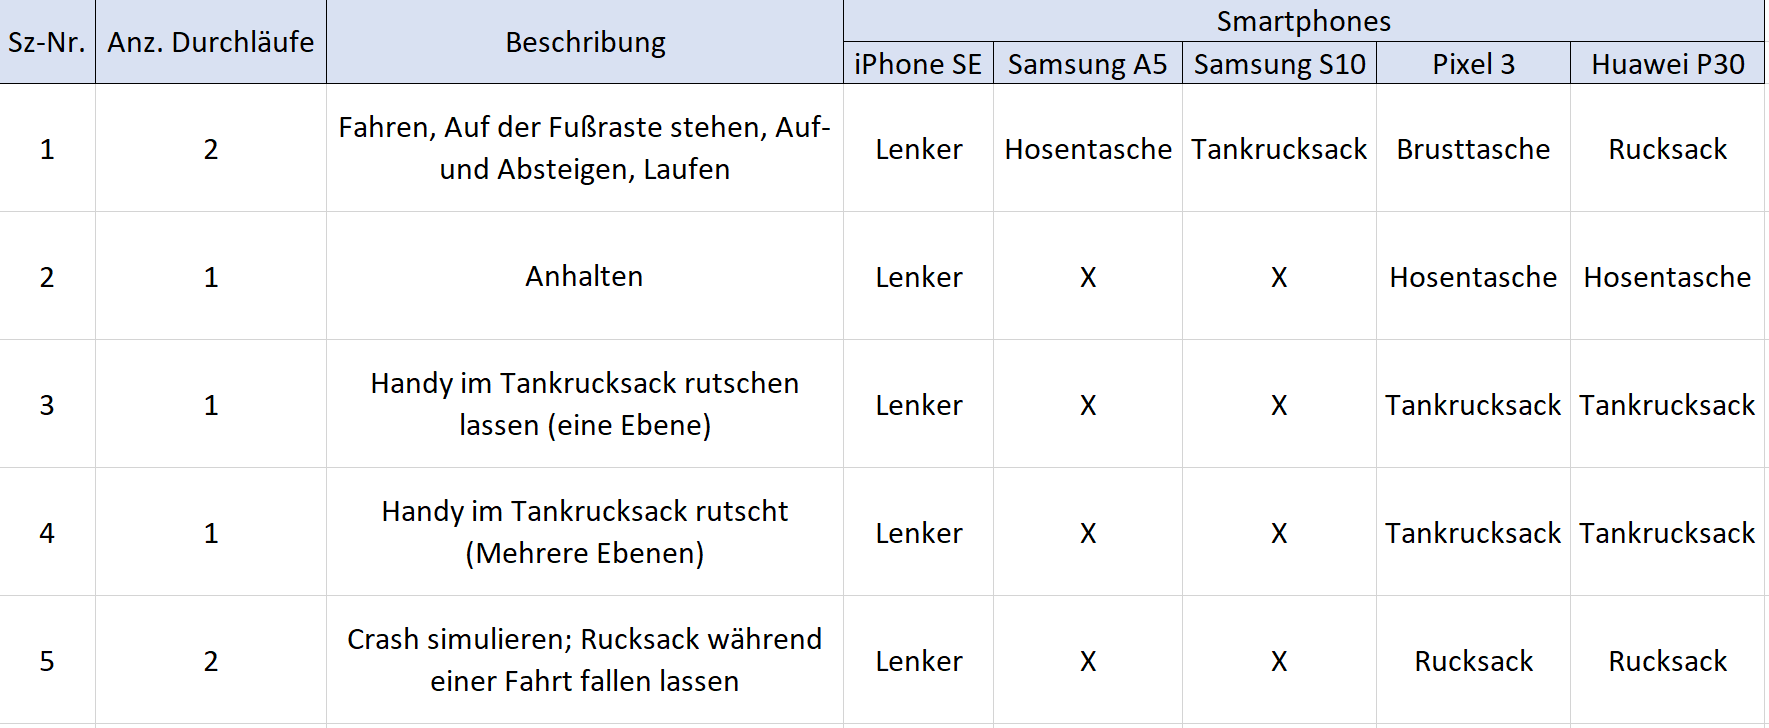
\includegraphics[width=\linewidth]{Bilder/TestSzenarienZusammenfassung.png} % TODO: Tabelle machen
%	\caption{Die Zusammenfassung der getesteten Szenarien}
%	\label{fig:TestSzenarienZusammenfassung}
%\end{figure}
\begin{landscape}
	\centering
	\begin{table}[htpb]	\footnotesize
		\caption{Die Zusammenfassung der getesteten Szenarien}
		\label{tab:TestSzenarienZusammenfassung}
		\begin{tabular}{|c|c|l|ccccc|}
			\hline
			\multirow{2}{*}{Sz-Nr} & \multirow{2}{*}{Anz. Durchläfe} & \multirow{2}{*}{Beschreibung} & \multicolumn{5}{c|}{Smartphones} \\ \cline{4-8} 
			&  & & \multicolumn{1}{c|}{iPhon SE} & \multicolumn{1}{c|}{Samsung A5} & \multicolumn{1}{c|}{Samsung S10} & \multicolumn{1}{c|}{Pixel 3} & Huawei P30 \\
			\hline
			1 & 2 & \begin{tabular}[c]{@{}l@{}}Fahrt,\\ Auf der Fußraste Stehen\\ Auf- und Absteigen\\ Laufen\end{tabular} & \multicolumn{1}{c|}{Lenker} & \multicolumn{1}{c|}{Hosentasche} & \multicolumn{1}{c|}{Tankrucksack} & \multicolumn{1}{c|}{Brusttasche} & Rucksack \\ 
			\hline
			2 & 1 & Anhalten & \multicolumn{1}{c|}{Lenker} & \multicolumn{1}{c|}{x} & \multicolumn{1}{c|}{x} & \multicolumn{1}{c|}{Hosentasche} & Hosentasche \\ 
			\hline
			3 & 1 & \begin{tabular}[c]{@{}l@{}}Handy im Tankrucksack\\ rutschen lassen (keine \\ Winkeländerung)\end{tabular} & \multicolumn{1}{c|}{Lenker} & \multicolumn{1}{c|}{x} & \multicolumn{1}{c|}{x} & \multicolumn{1}{c|}{Tankrucksack} & Tankrucksack \\ 
			\hline
			4 & 1 & \begin{tabular}[c]{@{}l@{}}Handy im Tankrucksack \\ rutschen lassen (Winkel-\\ änderung)\end{tabular} & \multicolumn{1}{c|}{Lenker} & \multicolumn{1}{c|}{x} & \multicolumn{1}{c|}{x} & \multicolumn{1}{c|}{Tankrucksack} & Tankrucksack \\ 
			\hline
			5 & 2 & \begin{tabular}[c]{@{}l@{}}Crash simulieren; \\ Rucksack während \\ einer Fahrt fallen lassen\end{tabular} & \multicolumn{1}{c|}{Lenker} & \multicolumn{1}{c|}{x} & \multicolumn{1}{c|}{x} & \multicolumn{1}{c|}{Rucksack} & Rucksack \\ 
			\hline
			
		\end{tabular}
	\end{table}
\end{landscape}

Der Versuchsablauf wird vor dem Testen vorbereitet und möglichst detailliert geplant, damit während des Testens kein Zeitverlust entsteht.
Demnächst werden die allgemeine Schritte des Versuchsablaufs aufgelistet.

\begin{itemize}
	\item[1] Befestigung und Einstellung der Kameras am Lenker und an der Brust, um die Wahrheit (Ground Truth) für die spätere Auswertung aufzunehmen
	\item[2] Befestigung der Smartphones (inklusive das Referenzhandy am Lenker) in der geplanten Stellen, Einschaltung und Prüfung der Signalaufnahme
	\item[3] Eine Kalibrierungsfahrt
	\item[4] Prüfung der Smartphoneskalibrierung
	\item[5] Start der Videoaufnahme und Dokumentation von Datum sowie Uhrzeit
	\item[6] Durchführung des Testversuchs (Variiert je nach dem Versuchsszenario)
	\item[7] Fahrtende und absteigen
	\item[8] Datenexport und -Übertragung
	\item[9] Datenexistenz im Zielordner prüfen
	\item[10] Löschung der Daten im Smartphone
	\item[11] Vorbereitung des nächsten Versuchs beziehungsweise Durchlaufs
\end{itemize}

Das erste Szenario ist das Wichtigste für diese Arbeit, weil dadurch die implementierte Lauferkennung sowie den Unterschied der Aktivitätserkennung zwischen den verschiedenen Bewegungsarten (z.B. Laufen, Fahren) getestet und verifiziert werden. Die einzelne Testschritte dieses Szenario werden hiermit erläutert:
\begin{itemize}
	\item Szenario 1: Fahrt mit verschiedener Fahrerpositionierung und Laufen sowie der Übergang dazwischen (Auf- und Absteigen)
	\begin{itemize}
		\item[1] Start der Videoaufnahme und Dokumentation von Datum sowie Uhrzeit
		\item[2] Normale Fahrt für ca. eine Minute
		\item[3] Fahrt in stehender Fahrerposition für ca. $10-20$ Sekunden
		\item[4] Normale Fahrt für ca. eine Minute
		\item[5] Anhalten und Absteigen
		\item[6] Laufen für $30-40$ Sekunden
		\item[7] Wieder Aufsteigen und eine normale Fahrt für ca. eine Minute
		\item[8] Fahrt in stehender Fahrerposition für ca. 10 Sekunden
		\item[9] Normale Fahrt für ca. eine Minute
		\item[10] Fahrtende und Fahrerabstieg
	\end{itemize}
\end{itemize}
Gleichzeitig werden die durch das integrierte Google-Tool erkannten Aktivitäten aufgenommen, damit diese mit der Ausgabe des implementierten Model \glqq Aktivitäts\-erke\-nnung\grqq{} verglichen werden. Das Ziel ist zu prüfen, ob es zuverlässiger wäre, das integrierte Tool zu verwenden.

% TODO: Figure mit verscshiedenen Screenshots hinzufügen, und die Einzelschritte des Szenarios zuordnen

\subsection{Referenz-Aktivitätsdaten (Ground truth)}

Die Lauferkennung beziehungsweise Aktivitätserkennung ergibt die Aussage (Fahren oder Laufen) und soll demnächst getestet werden. Für die Testung muss der tatsächliche Verlauf einer Fahrt bekannt werden. Zu diesem Zweck werden die Tests mit Videoaufnahmen nach der Durchführung optisch manuell mithilfe eines intern entwickelten LabVIEW-Tool ausgewertet. Diese Versuche sind mit Videos aufgenommen, die allerdings nur einen kleinen Teil der aufgezeichneten Signale abdecken. Damit die Videos dem richtigen Signalteil zugeordnet werden können, ist eine Synchronisierung zwischen dem Signal und dem dazugehörigen Video erforderlich. 

Der Benutzer kann mit dem internen Tool die Video-Signal-Synchronisierung unkompliziert erfolgen. Danach können bestimmte Labels (z.B. Fahren oder Stehen) für die entsprechenden Zeitfenster schnell und einfach eingegeben werden. Am Ende wird eine Tabelle exportiert, welche die gleiche originalen Daten sowie eine neue zusätzliche Spalte mit den Labels der Aktivitäten beinhaltet.
Diese Tabelle kann mit den Ergebnissen der Lauferkennung verglichen werden.

Die erwähnte Labels muss der Benutzer vorher definieren und in das Tool importieren. In der \autoref{tab:TabCalimotoLabelsID} ist die Tabelle der definierten Labels sichtbar. Die Tabelle hat sieben verschiedene Klassen, die sich im Tool mit den F-Tasten einfach eingeben lassen. \glqq Undefined\grqq{} entspricht unbekannter Eingabe, wenn das Motorrad nicht im Video sichtbar ist. \glqq Driving\grqq{} repräsentiert der Fahrt und \glqq Walking\grqq{} des Laufens.
 
In der \autoref{fig:Exporttabelle_Davilt} ist ein verkürztes Beispiel der exportierten Tabelle, in der die neue Spalte \glqq GroundTruthID\grqq{} sichtbar ist. In der Tabelle sind mehrere ausgeschnittene Phasen enthalten, die auch durch die GroundTruth-Daten unterschieden werden.
\begin{figure}
	\centering
	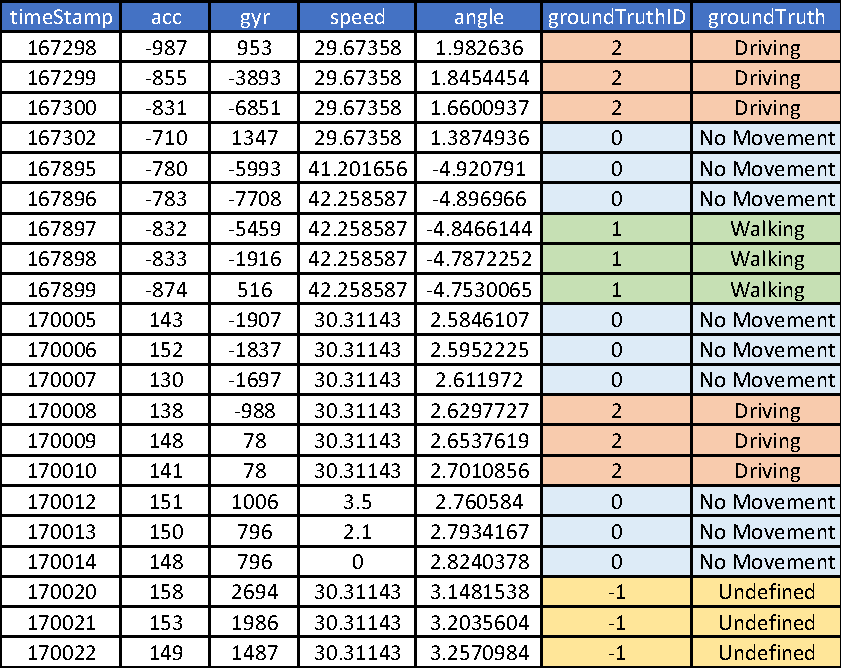
\includegraphics[width=\linewidth]{Bilder/GriundTruthTabelle.pdf}
	\caption{Beispiel der exportierten Tabelle mit der neuen Spalte}
	\label{fig:Exporttabelle_Davilt}
\end{figure}

%\begin{figure}
%	\centering
%	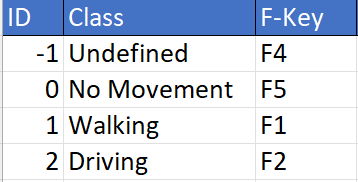
\includegraphics[width=0.6\linewidth]{Bilder/TabCalimotoLabelsID2.png} %TODO: Tabelle machen
%	\caption{Die definierte Labels von Groundtruth}
%	\label{fig:TabCalimotoLabelsID}
%\end{figure}

\begin{table}[]
	\caption{Die definierte Labels von Groundtruth}
	\label{tab:TabCalimotoLabelsID}
	\centering
		\begin{tabular}{|c|l|c|}
		\hline
		\textbf{ID} & \textbf{Class} & \textbf{F-Key} \\
		\hline
		-1 & Undefined & F4 \\ 
		\hline
		0 & No Movement & F5 \\ 
		\hline
		1 & Walking & F1 \\ 
		\hline
		2 & Driving & F2 \\ 
		\hline
	\end{tabular}
\end{table}














%\begin{table}\caption{Statistische Zahlen über Unfälle in Deutschland \cite{Verkehrsunfaelle_Fahrrad2017}} 
%	\centering
%	\begin{tabular}{|p{3.2cm}|>{\centering\arraybackslash}p{3.3cm}|>{\centering\arraybackslash}p{3.3cm}|>{\centering\arraybackslash}p{3.3cm}|}
	%		\hline
	%		\textbf{Jahr} & \textbf{Unfälle} & \textbf{Verunglückte} & \textbf{Getötete} \\
	%		\hline
	%		2000 & 382.949 & 511.577 & 7.503 \\
	%		\hline
	%		2005 & 336.619 & 438.804 & 5.361 \\
	%		\hline
	%		2010 & 288.297 & 374.818 & 3.648 \\
	%		\hline
	%		2014 & 302.435 & 392.912 & 3.377 \\
	%		\hline
	%		2015 & 305.659 & 396.891 & 3.459 \\
	%		\hline
	%		2016 & 308.145 & 399.872 & 3.206 \\
	%		\hline
	%		2017 & 302.656 & 393.492 & 3.180 \\
	%		\hline
	%	\end{tabular}
%	\label{tab:UnfallImJahren}
%\end{table}







